\ifdefined\COMPLETE
\else
    \input{./preambule-sacha-utf8.ltx}
    \begin{document}
\fi


\section{Intégration}

\subsection{Intégrale d'une fonction positive sur un intervalle}

\subsubsection{Unité d'aire}

Soit $\left(O\; ; \; \overrightarrow{i} \; ; \; \overrightarrow{j}\right)$ un repère \textbf{orthogonal}. \\
Soit $A$ le point défini par $\overrightarrow{OA} = \overrightarrow{i}$. \\
Soit $B$ le point défini par $\overrightarrow{OB} = \overrightarrow{j}$. \\

L'unité d'aire (ua) est l'aire du rectangle défini par les points $O$, $A$ et $B$, comme sur le dessin suivant : \\

\begin{tikzpicture}[line cap=round,line join=round,>=triangle 45,x=2cm,y=1cm,scale=.8]
\draw[->] (-0.5,0) -- (1.5,0);
\foreach \x in {1}
\draw[shift={(\x,0)}] (0pt,2pt) -- (0pt,-2pt) ; % node[below] {\footnotesize $\x$};
\draw (.5,0) node[below] {\footnotesize $\vec{i}$};
\draw (1,0) node[below] {\footnotesize $A$};

\draw[->] (0,-1.5) -- (0,2.5);
\foreach \y in {1}
\draw[shift={(0,\y)}] (2pt,0pt) -- (-2pt,0pt);  % node[left] {\footnotesize $\y$};
\draw (0pt,-8pt) node[left] {\footnotesize $0$};
\draw (0,.5) node[left] {\footnotesize $\vec{j}$};
\draw (0,1) node[left] {\footnotesize $B$};

\clip (-0.5,-1.5) rectangle (1.5,2.5);


\draw[pattern=north east lines, pattern color=blue] (0,0) rectangle (1,1) ; 
\draw [fill=white] (0,0) rectangle (.125,.25) ; 



\begin{pgfonlayer}{background}   
\draw[step=1mm,ultra thin,AntiqueWhite!10] (-0.5,-1.5) grid (1.5,2.5);
\draw[step=5mm,very thin,AntiqueWhite!30] (-0.5,-1.5) grid (1.5,2.5);
\draw[step=1cm,very thin,AntiqueWhite!50]  (-0.5,-1.5) grid (1.5,2.5);
\draw[step=5cm,thin,AntiqueWhite]           ((-0.5,-1.5) grid (1.5,2.5);
\end{pgfonlayer}

\end{tikzpicture}

\subsubsection{Définition}

Soit $f$ une fonction continue et positive sur un intervalle $\left[a \; ; \; b\right]$. \\ 
Soit $C_f$ ma représentation graphique de $f$ dans un repère orthonormal $\left(O\; ; \; \overrightarrow{i} \; ; \; \overrightarrow{j}\right)$. \\

L'intégrale entre $a$ et $b$ de $f$, notée $\displaystyle \int_a^b f(x) \; \mathrm{dx}$ est l'aire, en unité d'aire, de la portion de plan délimitée par $C_f$, l'axe des abscisses, la droite d'équation $x = a$ et la droite d'équation $x = b$. \\

\begin{tikzpicture}[line cap=round,line join=round,>=triangle 45,x=2cm,y=1cm,scale=1]
\draw[->] (-0.5,0) -- (2.5,0);

\draw (.5,0) node[below] {\footnotesize $a$}; \draw (.5,3.2) node[above] {\footnotesize $x=a$}; 
\draw (2,0) node[below] {\footnotesize $b$};  \draw (2,3.2) node[above] {\footnotesize $x=b$}; 

\draw[->] (0,-1.5) -- (0,3.5);

\draw (0pt,-8pt) node[left] {\footnotesize $0$};


\clip (-0.5,-1) rectangle (2.6,4);

\draw(.5,0) -- (.5,3.2) ; 
\draw(2,0) -- (2,3.2) ; 

\draw [fill=white] (0,0) rectangle (.125,.25) ; 

\draw (2,2.2) node[right] {\footnotesize $\mathcal{C}_f $};

\draw [smooth, samples=100,domain=0.2:2.5]  plot(\x,{(26/15)*(\x)^3 -(31/5)*(\x)^2 +(20/3)*(\x) -(1/5)}) ; 

\fill [pattern=north east lines, smooth, samples=100,domain=0.5:2] (0.5,0) -- (.5, 1.8) -- plot(\x,{(26/15)*(\x)^3 -(31/5)*(\x)^2 +(20/3)*(\x) -(1/5)}) -- (2,2.2) -- (2,0) -- cycle ;

\begin{pgfonlayer}{background}   
\draw[step=1mm,ultra thin,AntiqueWhite!10] (-0.5,-1) grid (2.6,4);
\draw[step=5mm,very thin,AntiqueWhite!30] (-0.5,-1) grid (2.6,4);
\draw[step=1cm,very thin,AntiqueWhite!50]  (-0.5,-1) grid (2.6,4);
\draw[step=5cm,thin,AntiqueWhite]           (-0.5,-1) grid (2.6,4);
\end{pgfonlayer}

\end{tikzpicture}

\vspace*{.3cm}

$\displaystyle \int_a^b f(x) \; \mathrm{dx}$ est lue « intégrale de $a$ à $b$ de $f(x)$ dx », où $a$ est la borne inférieure et $b$ la borne supérieure de l'intégrale. \\

\textbf{Remarque :} $x$ est une lettre muette. On a donc $\displaystyle \int_a^b f(x) \; \mathrm{dx} = \displaystyle \int_a^b f(t) \; \mathrm{dt}$. \\

\newpage

\textbf{Exemple :} \\

\begin{tabular}{llll}
Soit la fonction $f:$ & $\R$ & $\longrightarrow$ & $\R$ \\
& $x$ & $\longmapsto$ & $f(x) = x+1$. \\
\end{tabular}

\vspace*{.3cm}

On a $D_f = \R$. \\

La fonction est représentée ainsi : \\

\begin{tabular}{ll}

\begin{tikzpicture}[line cap=round,line join=round,>=triangle 45,x=1cm,y=1cm,scale=1]
\draw[->] (-0.5,0) -- (8,0);
\foreach \x in {1,...,7}
\draw[shift={(\x,0)}] (0pt,2pt) -- (0pt,-2pt) ; % node[below] {\footnotesize $\x$};
\draw (1,0) node[below] {\footnotesize $1$}; \draw (1,9.5) node[above] {\footnotesize $x=1$}; 
\draw (7,0) node[below] {\footnotesize $7$};  \draw (7,9.5) node[above] {\footnotesize $x=7$}; 

\draw[->] (0,-0.5) -- (0,10);
\foreach \y in {1,...,10}
\draw[shift={(0,\y)}] (2pt,0pt) -- (-2pt,0pt);  % node[left] {\footnotesize $\y$};
\draw (0pt,-8pt) node[left] {\footnotesize $0$};
\draw (0,2) node[left] {\footnotesize $2$};
\draw (0,8) node[left] {\footnotesize $8$};

\clip (-0.5,-.5) rectangle (9,12);

\draw(1,0) -- (1,9.5) ; 
\draw(7,0) -- (7,9.5) ; 
\draw [dashed]  (0,8) -- (7,8) ; 

\draw [smooth, samples=100,domain=-1:8]  plot(\x,{(\x)+1)}) ; 

\fill [pattern=north west lines, smooth, samples=100,domain=1:7] (1,0) -- (1,2) -- plot(\x,{(\x)+1}) -- (7,8) -- (7,0) -- cycle ;

\begin{pgfonlayer}{background}   
\draw[step=1mm,ultra thin,AntiqueWhite!10] (-0.5,-.5) grid (9,12) ;
\draw[step=5mm,very thin,AntiqueWhite!30] (-0.5,-.5) grid (9,12) ;
\draw[step=1cm,very thin,AntiqueWhite!50]  (-0.5,-.5) grid (9,12) ;
\draw[step=5cm,thin,AntiqueWhite]           (-0.5,-.5) grid (9,12) ;
\end{pgfonlayer}

\end{tikzpicture}

& 

\begin{minipage}{5cm}
\vspace*{-13cm}
On cherche à calculer $\mathcal{A} = \displaystyle \int_1^7 f(x) \; \mathrm{dx}$. \\

$\mathcal{A}$ est la somme des aires du rectangle de largeur $2$ et de longueur $7$ et du triangle rectangle restant. \\

On a $\mathcal{A} = 6 \times 2 + \dfrac{1}{2} \times 6 \times 6 = 30$. \\

D'où $\mathcal{A} = 30 ua$. \\

\begin{itemize}
\item[•] Si l'unité de longueur est un grand carreau, soit $0,8$ cm, alors $\mathcal{A} = 30 \times 0,64 \mathrm{cm}^2 = 19,2 \mathrm{cm}^2$. \\
\item[•] Si l'unité de longueur est deux petits carreaux, soit $1$ cm, alors $\mathcal{A} = 30 \times 1 \mathrm{cm}^2 = 1 \mathrm{cm}^2$. \\
\end{itemize}

\vspace*{.3cm}

Donc $\displaystyle \int_1^7 \left(x+1\right) \; \mathrm{dx} = 30$. 
\end{minipage}

\end{tabular}

\subsubsection{Conséquences immédiates}

Soit $f$ une fonction continue et positive sur un intervalle $\left[a \; ; \; b\right]$. \\

On a :

\vspace*{-.5cm}

\begin{tabular}{ll}

\begin{minipage}{10cm}
\begin{itemize}
\item[•] $\displaystyle \int_a^b f(x) \; \mathrm{dx}$ est un nombre positif. \\
\item[•] $\displaystyle \int_a^a f(x) \; \mathrm{dx} = 0$ \\
\item[•] $\displaystyle \int_a^b f(x) \; \mathrm{dx} = \displaystyle \int_a^c f(x) \; \mathrm{dx} + \displaystyle \int_c^b f(x) \; \mathrm{dx}$ \\
\end{itemize}

Cette troisième relation est appelée « relation de Chasles » pour les intégrales, et peut-être représentée par le dessin ci-contre : 
\end{minipage}
&
\begin{minipage}{5cm}
\begin{tikzpicture}[line cap=round,line join=round,>=triangle 45,x=2cm,y=1cm,scale=1]
\draw[->] (-0.5,0) -- (2.5,0); \draw[->] (0,0) -- (0.35,0);
% \foreach \x in {1}
% \draw[shift={(\x,0)}] (0pt,2pt) -- (0pt,-2pt) ; % node[below] {\footnotesize $\x$};

\draw (.5,0) node[below] {\footnotesize $a$} ; 
\draw (1,0) node[below] {\footnotesize $c$} ; 
\draw (2,0) node[below] {\footnotesize $b$} ; 

\draw[->] (0,-1.5) -- (0,3.5);
\draw[->] (0,0) -- (0,1);
% \foreach \y in {1}
% \draw[shift={(0,\y)}] (2pt,0pt) -- (-2pt,0pt);  % node[left] {\footnotesize $\y$};
\draw (0pt,-8pt) node[left] {\footnotesize $0$};
% \draw (0,.5) node[left] {\footnotesize $\vec{i}$};
% \draw (0,1) node[left] {\footnotesize $B$};

\clip (-0.5,-1) rectangle (2.6,4);

\draw(.5,0) -- (.5,1.7) ; 
\draw  (1,0) -- (1,2) ; 
\draw(2,0) -- (2,2.2) ; 

% \draw[pattern=north east lines, pattern color=blue] (0,0) rectangle (1,1) ; 
\draw [fill=white] (0,0) rectangle (.125,.25) ; 

% \draw (2,2.2) node[right] {\footnotesize $\mathcal{C}_f $};

\draw [smooth, samples=100,domain=0.2:2.2]  plot(\x,{(26/15)*(\x)^3 -(31/5)*(\x)^2 +(20/3)*(\x) -(1/5)}) ; 

\fill [pattern=north west lines, smooth, samples=100,domain=0.5:1] (0.5,0) -- (.5, 1.8) -- plot(\x,{(26/15)*(\x)^3 -(31/5)*(\x)^2 +(20/3)*(\x) -(1/5)}) -- (1,1.7) -- (1,0) -- cycle ;
\fill [pattern=north east lines, smooth, samples=100,domain=1:2] (1,0) -- (1, 1.7) -- plot(\x,{(26/15)*(\x)^3 -(31/5)*(\x)^2 +(20/3)*(\x) -(1/5)}) -- (2,2.2) -- (2,0) -- cycle ;

\begin{pgfonlayer}{background}   
\draw[step=1mm,ultra thin,AntiqueWhite!10] (-0.5,-1) grid (2.6,4);
\draw[step=5mm,very thin,AntiqueWhite!30] (-0.5,-1) grid (2.6,4);
\draw[step=1cm,very thin,AntiqueWhite!50]  (-0.5,-1) grid (2.6,4);
\draw[step=5cm,thin,AntiqueWhite]           (-0.5,-1) grid (2.6,4);
\end{pgfonlayer}
\end{tikzpicture}
\end{minipage}
\\
\end{tabular}

\vspace*{-5cm}

\newpage

\vspace*{-1.7cm}

\subsection{Notion de primitives}

\subsubsection{Théorème fondamental}

Soit $f$ une fonction continue et positive sur un intervalle $\left[a \; ; \; b\right]$. \\

La fonction $F\left(x\right) = \displaystyle \int_a^b f(t) \; \mathrm{dt}$ est dérivable sur $\left[a \; ; \; b\right]$ et pour tout $x \in \left[a \; ; \; b\right], F'(x) = f(x)$. \\
On dit que $F$ est \underline{\textbf{une} primitive} de $f$ sur $\left[a \; ; \; b\right]$.

\subsubsection{Exemple}

\begin{tabular}{llll}
Soit la fonction $f:$ & $\R$ & $\longrightarrow$ & $\R$ \\
& $x$ & $\longmapsto$ & $f(x) = 2x$. \\
\end{tabular}

\vspace*{.3cm}

\begin{tabular}{ll}

\begin{minipage}{3.5cm}

\begin{tikzpicture}[line cap=round,line join=round,>=triangle 45,x=1cm,y=1cm,scale=1]
\draw[->] (-0.5,0) -- (3,0);
\foreach \x in {1}
\draw[shift={(\x,0)}] (0pt,2pt) -- (0pt,-2pt)  node[below] {\footnotesize $\x$};
% \draw (1,0) node[below] {\footnotesize $1$}; \draw (1,9.5) node[above] {\footnotesize $x=1$}; 
% \draw (7,0) node[below] {\footnotesize $7$};  \draw (7,9.5) node[above] {\footnotesize $x=7$}; 
 \draw (1.7,0) node[below] {\footnotesize $x$}; 
\draw[->] (0,-0.5) -- (0,3.7);
\foreach \y in {1,...,5}
\draw[shift={(0,1)}] (2pt,0pt) -- (-2pt,0pt)  node[left] {\footnotesize $1$};
\draw[shift={(0,2)}] (2pt,0pt) -- (-2pt,0pt)  node[left] {\footnotesize $2$};`
\draw[shift={(0,3)}] (2pt,0pt) -- (-2pt,0pt)  node[left] {\footnotesize $3$};
\draw[shift={(0,3.4)}] (2pt,0pt) -- (-2pt,0pt)  node[left] {\footnotesize $2x$};

\clip (-0.5,-.5) rectangle (3,4);

\draw (0,0) -- (3,6) ; 
\draw [dashed] (0,3.4) -- (1.7,3.4) -- (1.7,0) ; 

\begin{pgfonlayer}{background}   
\draw[step=1mm,ultra thin,AntiqueWhite!10] (-0.5,-.5) grid (3,4) ;
\draw[step=5mm,very thin,AntiqueWhite!30] (-0.5,-.5) grid (3,4) ;
\draw[step=1cm,very thin,AntiqueWhite!50]  (-0.5,-.5) grid (3,4) ;
\draw[step=5cm,thin,AntiqueWhite]           (-0.5,-.5) grid (3,4) ;
\end{pgfonlayer}

\end{tikzpicture}

\end{minipage}

&

\begin{minipage}{7cm}

\vspace*{.3cm}

On a $D_f = \R$. \\

On a $\displaystyle \int_0^x f(t) \; \mathrm{dt} = \dfrac{1}{2}x \times 2x = x^2$. \\

On a aussi $F(x) = x^2$, car $F'(x) = 2x = f(x)$. 

\end{minipage}

\\

\end{tabular}

\subsubsection{Théorème}

Soit $f$ la fonction continue et positive sur l'intervalle $\left[a \; ; \; b\right]$. 

La fonction $f$ définie par $F(x) = \displaystyle \int_a^x f(t) \; \mathrm{dt}$ est dérivable sur $\left[a \; ; \; b\right]$ et pour tout $x \in \left[a \; ; \; b\right], F'(x) = f(x)$. \\

$F$ est \textbf{une} primitive de $f$ sur l'intervalle $\left[a \; ; \; b\right]$. \\

\begin{tabular}{ll}

\begin{minipage}{8cm}

\begin{tikzpicture}[line cap=round,line join=round,>=triangle 45,x=1.2cm,y=1.3cm]
\draw[->,color=black] (1.5,1) -- (6.82,1);
% \foreach \x in {,1,2,3,4,5,6}
%\draw[shift={(\x,0)},color=black] (0pt,2pt) -- (0pt,-2pt) ; % node[below] {\footnotesize $\x$};
\draw[->,color=black] (2,0.5) -- (2,3.95);
%\foreach \y in {1,2,3}
%\draw[shift={(0,\y)},color=black] (2pt,0pt) -- (-2pt,0pt); % node[left] {\footnotesize $\y$};
%  \draw[color=black] (0pt,-10pt) node[right] {\footnotesize $0$};
\clip (1,.5) rectangle (7,4.4);

\draw[color=blue,smooth,samples=100,domain=2.8:5.2] plot(\x,{-0.1*(\x)*(\x)*(\x)+1.03*(\x)*(\x)-2.85*(\x)+4.07});

\fill [pattern=north west lines,smooth,samples=100,domain=3:5] (3,1)  -- (3, 2.1)  plot(\x,{-0.1*(\x)*(\x)*(\x)+1.03*(\x)*(\x)-2.85*(\x)+4.07}) -- (5,3.07) --   (5,1) --  (3,1)  -- cycle  ; 

\draw [dashed] (3,1)  node [below] {\footnotesize $x_0$}      -- (3, 2.1) -- (2,2.1)  node [left] {\footnotesize $f(x_0)$} ;
\draw [dashed] (5,1)  node [below] {\footnotesize $x_0 + h$} -- (5, 3.07) -- (2,3.07)  node [left] {\footnotesize $f(x_0+h)$} ;


\begin{pgfonlayer}{background}   
\draw[step=1mm,ultra thin,AntiqueWhite!10]  (1,.5) grid (7,4.4) ;
\draw[step=5mm,very thin,AntiqueWhite!30]  (1,.5) grid (7,4.4) ;
\draw[step=1cm,very thin,AntiqueWhite!50]   (1,.5) grid (7,4.4) ;
\draw[step=5cm,thin,AntiqueWhite]            (1,.5) grid (7,4.4) ;
\end{pgfonlayer}

\end{tikzpicture}

\end{minipage}

&

\begin{minipage}{7cm}
$ \mathcal{A} = \displaystyle \int_{x_0}^{x_0+h} f(t) \; \mathrm{dt} \approx h \times f(x_0)$. \\

On a $h$ est la longueur de la portion de plan et $f(x_0)$ est la hauteur de portion de plan. \\

\end{minipage}

\end{tabular}

%\vspace*{-.5cm}

\begin{tabular}{lll}
On a $\displaystyle \int_a^{x_0+h} f(t) \; \mathrm{dt} = \displaystyle \int_a^{x_0} f(t) \; \mathrm{dt} + \displaystyle \int_{x_0}^{x_0 + h} f(t) \; \mathrm{dt}$ & $\Longleftrightarrow$ & $F\left(x_0 + h\right) = F\left(x_0\right) +  \displaystyle \int_{x_0}^{x_0 + h} f(t) \; \mathrm{dt}$ \vspace*{.3cm} \\
& $\Longleftrightarrow$ & $F\left(x_0+h\right) - F\left(x_0\right) = \displaystyle \int_{x_0}^{x_0 + h} f(t) \; \mathrm{dt}$ \vspace*{.3cm} \\
& $\Longleftrightarrow$ & $F\left(x_0+h\right) - F\left(x_0\right) \approx hf\left(x_0\right)$. \\
\end{tabular} 

\vspace*{.3cm}

En divisant par $h$ de chaque côté de l'équation, on a : $\underbrace{\dfrac{F\left(x_0+h\right) - F\left(x_0\right)}{h}}_{\mathrm{Taux \; de \; variations \; de \; F, \\ noté \;} T(h)} \approx \; \; \; \; \;  \; \; \underbrace{\dfrac{hf\left(x_0\right)}{h}}_{f\left(x_0\right)}$.

D'où $T(h) \approx f\left(x_0\right)$.

\vspace*{-5cm}

\newpage

\vspace*{-1.5cm}

\textbf{Rappel :} \\

\begin{tabular}{llll}
\hspace{-.3cm} Soit la fonction $f :$ & $\R$ & $\longrightarrow$ & $\R$ \\
& $f$ & $\longmapsto$ & $f(x) = x^2$ \\
\end{tabular}

On a $D_f = \R$. \\

Soit $x_0 \in D_f$. \\

Montrons que $f$ est dérivable en $x_0$. \\

\begin{itemize}
\item[•] Calcul du taux d'accroissement : \vspace*{.3cm}
\\
\begin{tabular}{llll}
$T(h)$ & $=$ & $\dfrac{f(x_0 + h) - f(x_0)}{h}$ & \vspace*{.3cm} \\
& $=$ & $\dfrac{\left(x_0 + h\right)^2 - x_0^2}{h}$ & \vspace*{.3cm} \\
& $=$ & $\dfrac{x_0^2 + 2x_0h + h^2 - x_0^2}{h}$ & \vspace*{.3cm} \\
& $=$ & $\dfrac{2x_0h + h^2}{h}$ & \vspace*{.3cm} \\
& $=$ & $\dfrac{h\left(2x_0 + h\right)}{h}$ & \vspace*{.3cm} \\
& $=$ & $2x_0 + h$ & si $h \neq 0$ \\
\end{tabular} \\
\vspace*{.3cm}

\item[•] Limite du taux d'accroissement : \vspace*{.3cm}

$\lim\limits_{h \to 0} T(h) = \lim\limits_{h \to 0} (2x_0 + h) = 2x_0$ \vspace*{.3cm} \\

Donc $f$ est dérivable en $x_0$ et $f'(x_0) = 2x_0$. \\

\item[•] Fonction dérivée : \\

\begin{tabular}{llllll}
$f' :$ & $\R$ & $\longrightarrow$ & $\R$ & & \\
& $x_0$ & $\longmapsto$ & $f'(x_0)$ & $ = $ & $2x_0$ \\
& $x$ & $\longmapsto$ & $f'(x)$ & $ = $ & $2x$ \\
\end{tabular}
\end{itemize}

\vspace*{.3cm}

On a $D_{f'} = \R$. \\

$f$ est une primitive de la fonction $f'$. 

\newpage

\vspace*{-2.2cm}

\subsection{Primitives d'une fonction sur un intervalle}

\subsubsection{Définition}

Soit $f$ une fonction définie sur un intervalle $I$. \\
$F$ est \textbf{une} primitive de $f$ sur $I$ si et seulement si $\left\{
  \begin{array}{l}
   F \mathrm{ \; est \; dérivable \; sur \; } I.\\
    \mathrm{pour \; tout \; } x \in I, F'(x) = f(x). \\
  \end{array}
\right.$

\vspace*{.3cm}

\textbf{Exemple :} \\

\begin{tabular}{llll}
\hspace*{-.3cm} Soit la fonction $F:$ & $\R$ & $\longrightarrow$ & $\R$ \\
& $x$ & $\longmapsto$ & $F(x) = \dfrac{1}{3}x^3 - x^2 - 3x + 5$ \\
\end{tabular}

\vspace*{.3cm}

\begin{tabular}{llll}
\hspace*{-.3cm} Soit la fonction $f:$ & $\R$ & $\longrightarrow$ & $\R$ \\
& $x$ & $\longmapsto$ & $f(x) = x^2 - 2x - 3$\\
\end{tabular}

\vspace*{.3cm}

On a $D_F = D_f = \R$. \\

On a aussi $F'(x) = x^2 - 2x - 3$. \\

D'où $\forall x \in \R, F'(x) = f(x)$. \\

Donc $F$ est \textbf{une} primitive de $f$ sur $\R$. 

\subsubsection{Propriétés}

Soit $f$ une fonction définie sur un intervalle $I$. \\ Soit $F$ une primitive de $f$ sur $\R$. \\

\begin{itemize}
\item[1.] L'ensemble \hbox{des primitives de $f$ sur I est constitué par les fonctions $\phi$ telles que pour tout $x \in I$,} \\ $\phi\left(x\right) = F(x) + k$, avec $k$ une constante quelconque. \\

\textbf{Démonstration : } \\

\textbf{Première partie : dans le sens direct} 

On a $\phi\left(x\right) = F\left(x\right) + k$. 

D'où $\phi'\left(x\right) = F'(x) + 0 = f(x)$. 

Donc $\phi$ est une primitive de $f$ sur $I$. \\

\textbf{Seconde partie : Réciproquement} 

Soit $\phi$ une primitive de $f$ sur $I$. \\

\begin{tabular}{lll}
\hspace{-.3cm} On a pour tout $x \in I$, $\phi'\left(x\right) = f\left(x\right)$ & $\Longleftrightarrow$ & $\phi'\left(x\right) = F'\left(x\right)$ \\
& $\Longleftrightarrow$ & $\phi'\left(x\right) - F'\left(x\right) = 0$ \\
& $\Longleftrightarrow$ & $\left(\phi' - F'\right)\left(x\right) = 0$ \\
& $\Longleftrightarrow$ & $\left(\phi - F\right)'\left(x\right) = 0$ \\
& $\Longleftrightarrow$ & $\left(\phi - F\right)\left(x\right) = k$ \\
& $\Longleftrightarrow$ & $\phi\left(x\right) - F\left(x\right) = k$ \\
& $\Longleftrightarrow$ & $\phi\left(x\right) = F\left(x\right) + k$ \\
\end{tabular}

\vspace*{.3cm}

\item[2.] Soit $x_0 \in I$ et soit $y_0 \in \R$. \\

Il existe \textbf{une et une seule primitive de } $\mathbf{f}$ sur $I$ tel que $\phi\left(x_0\right) = y_0$. \\

En effet, on a $ \phi\left(x_0\right) = y_0 \Longleftrightarrow F\left(x_0\right) + k = y_0 \Longleftrightarrow k = y_0 - F(x_0)$
\end{itemize}

\newpage

\subsubsection{Exercices}

\textbf{Exercice n°1} \\

\begin{tabular}{llll}
Soit la fonction $f:$ & $\R$ & $\longrightarrow$ & $\R$ \\
& $x$ & $\longmapsto$ & $f(x) = \left(x-1\right)e^x + 2$ \\
\end{tabular}

\vspace*{.3cm}

\begin{itemize}
\item[1.] Montrer que la fonction $F$ définie par $F(x) = \left(x-2\right)e^x + 2x$ est \textbf{une} primitive de $f$ sur $\R$. \\
\item[2.] Déterminer \textbf{la} primitive $\phi$ de $f$ sur $\R$ telle que $\phi\left(1\right) = 2$ \\
\end{itemize}

\vspace*{.3cm}

1. On a $F(x) = \left(x-2\right)e^x + 2x$. \\

\begin{tabular}{llll}
Ainsi, $\forall x \in \R$, & $F'(x)$ & $=$ & $1 \times e^x + \left(x-2\right)e^x + 2$ \\
& & $=$ & $e^x + \left(x-2\right)e^x + 2$ \\
& & $=$ & $\left(1 + x - 2\right)e^x + 2$ \\
& & $=$ & $\left(x-1\right)e^x + 2$ \\
\end{tabular}

Ainsi, $\forall x \in \R$, $F'(x) = f(x)$. Donc $F$ est une primitive de $f$ sur $\R$. \\

2. $\phi\left(x\right) = F\left(x\right) + k$. \\

Donc $\phi\left(x\right) = \left(x-2\right)e^x + 2x + k$. \\

Or, $\phi\left(1\right) = 2$. \\

\begin{tabular}{lll}
\hspace{-.3cm} D'où, $-1e^1 + 2 + k = 2$ & $\Longleftrightarrow$ & $-e + 2 + k = 2$ \\
& $\Longleftrightarrow$ & $k - e = 0$ \\
& $\Longleftrightarrow$ & $k = e$ \\
\end{tabular}

D'où $\phi\left(x\right) = \left(x-2\right)e^x + 2x + e$ est \textbf{la} primitive cherchée. \\

\newpage

\textbf{Exercice n°2} \\

\begin{tabular}{llll}
\hspace{-.3cm} Soit la fonction $f:$ & $\R$ & $\longrightarrow$ & $\R$ \\
& $x$ & $\longmapsto$ & $f(x) = \ln x - \ln\left(-x + 4\right)$ \\
\end{tabular}

\vspace*{.3cm}

\begin{itemize}
\item[1.] Déterminer $D_f$. \\
\item[2.] Montrer que \hbox{la fonction $F$ définie par $F(x) = x\ln x + \left(-x + 4\right)\ln\left(-x + 4\right)$ est \textbf{une} primitive de $f$ sur $\left[1 \; ; \; 3\right]$.} \\
\item[3.] Déterminer \textbf{la} primitive $\phi$ de $f$ sur $\left[1 \; ; \; 3\right]$ telle que $\phi\left(3\right) = 0$ \\
\end{itemize}

\vspace*{.3cm}

1. Il faut que $\left\{
  \begin{array}{rll}
    x & > & 0 \\
    -x+4 & > & 0 \\
  \end{array}
\right. \Longleftrightarrow \left\{
  \begin{array}{rll}
    x & > & 0 \\
    x & < & 4 \\
  \end{array}
\right.$ \vspace*{.3cm} \\

D'où $D_f = \left]0 \; ; \; 4\right[$. \\

\textbf{Remarque :} On a $\left[1 \; ; \; 3\right] \subset \left] 0 \; ; \; 4\right[$. \\

On raisonnera par la suite dans $\left[1 \; ; \; 3\right]$ afin de raisonner dans un intervalle fermé. \\

2. On a $F(x) = x\ln x + \left(-x + 4\right)\ln\left(-x + 4\right)$. \\

\begin{tabular}{llll}
Ainsi, $\forall x \in \left[1 \; ; \; 3\right]$, & $F'(x)$ & $=$ & $1 \times \ln x + x \times \dfrac{1}{x}  -1\left[\ln\left(-x + 4\right)\right] + \left(-x + 4\right) \left(\dfrac{-1}{-x + 4}\right)$ \vspace*{.3cm} \\
& & $=$ & $\ln x + 1 -\ln\left(-x + 4\right) - 1$ \\
& & $=$ & $\ln x -\ln\left(-x + 4\right)$ \\
\end{tabular}

\vspace*{.3cm}

Ainsi, $\forall x \in \R$, $F'(x) = f(x)$. Donc $F$ est une primitive de $f$ sur $\left[1 \; ; \; 3\right]$. \\

3. $\phi\left(x\right) = F\left(x\right) + k$. \\

Donc $\phi\left(x\right) = x\ln x + \left(-x + 4\right)\ln\left(-x + 4\right) + k$. \\

Or, $\phi\left(3\right) = 0$. \\

\begin{tabular}{lll}
\hspace{-.3cm} D'où, $3 \ln 3 + \left(-3 + 4\right)\ln\left(-3 + 4\right) + k = 0$ & $\Longleftrightarrow$ & $3 \ln 3 + 1 \times 0 + k = 0$ \\
& $\Longleftrightarrow$ & $3 \ln 3 + k = 0$ \\
& $\Longleftrightarrow$ & $k = -3\ln 3$ \\
\end{tabular}

\vspace*{.3cm}

D'où $\phi\left(x\right) = x\ln x + \left(-x + 4\right)\ln\left(-x + 4\right) - 3\ln 3$ est \textbf{la} primitive cherchée. \\

\newpage

\vspace*{-2cm}

\subsection{Calculs de primitives}

\subsubsection{Fonctions continues sur un intervalle}

\textbf{Théorèmes :} \\

\begin{itemize}
\item[•] Tout fonction continue et positive sur un intervalle $\left[a \; ; \; b\right]$ admet une primitive sur $\left[a \; ; \; b\right]$ et donc une infinité de primitives sur $\left[a \; ; \; b\right]$. \\

Soit $f$ une fonction continue et positive sur $\left[a \; ; \; b \right]$. La fonction $F$ définie par $F\left(x\right) = \displaystyle \int_a^b f(t) \; \mathrm{dt}$ est une primitive de $f$ sur $\left[a \; ; \; b\right]$. \\

\item[•] Plus généralement, on admet que tout donction continue sur un intervalle $\left[a \; ; \; b\right]$ admet une primitive sur $\left[a \; ; \; b\right]$ et donc une infinité de primitives sur $\left[a \; ; \; b\right]$
\end{itemize}

%\vspace*{.3cm}

\begin{tabular}{ll}
\begin{minipage}{8cm}

\textbf{Exemple n°1} \\

\begin{tabular}{llll}
Soit la fonction $f:$ & $\R$ & $\longrightarrow$ & $\R$ \\
& $x$ & $\longmapsto$ & $f\left(x\right) = e^x$ \\
\end{tabular}

\vspace*{.3cm}

On a $D_f = \R$. \\

$f$ est continue sur $\R$. \\ Donc $f$ admet une primitive sur $\R$ et donc une infinité de primitives sur $\R$. \\

On a $F(x) = e^x$ et $\phi\left(x\right) = e^x + k$. \\
\end{minipage}
&
\begin{minipage}{5cm}
\begin{tikzpicture}[line cap=round,line join=round,>=triangle 45,x=1.0cm,y=1.0cm,scale=.9]
\draw[->] (-3.5,0) -- (5.5,0);
\foreach \x in {-3,-2,-1,1,2,3,4,5}
\draw[shift={(\x,0)}] (0pt,2pt) -- (0pt,-2pt) node[below] {\footnotesize $\x$};
\draw[->] (0,-2.14) -- (0,6);
\foreach \y in {-2,-1,1,2,3,4,5,6}
\draw[shift={(0,\y)}] (2pt,0pt) -- (-2pt,0pt) node[left] {\footnotesize $\y$};
\draw (0pt,-10pt) node[right] {\footnotesize $0$};
\clip(-3.5,-2.14) rectangle (6,6);

\draw [domain=-7:4,blue] plot(\x,{exp(\x*ln(e)}) ; 

\foreach \x in {2}
\draw [color=blue] (\x,{exp(\x*ln(e)}) -- ++(-1.5pt,-1.5pt) -- ++(3.0pt,3.0pt) ++(-3.0pt,0) -- ++(3.0pt,-3.0pt);

\foreach \x in {0,1}
\draw [color=red] (\x,{exp(\x*ln(e)}) -- ++(-1.5pt,-1.5pt) -- ++(3.0pt,3.0pt) ++(-3.0pt,0) -- ++(3.0pt,-3.0pt);
\draw [red] (0,1) node [right] { $I$} ; 
\draw [red] (0,e) node [left] { $e$} ; 
\draw [red] (1,e) node [right] { $J$} ; 
\draw [red, dashed] (0,e) -- (1,e) ; 
\draw [DarkGreen] (-.8,0.2) -- (1, 2) ;
\draw [<->, DarkGreen] (-.5,.5) -- (.5,1.5) ; 
\draw [DarkGreen] (0,0) -- (7,7) ; 

\begin{pgfonlayer}{background}   
\draw[step=1mm,ultra thin,AntiqueWhite!10] (-3.5,-2.14) grid (6,6);
\draw[step=5mm,very thin,AntiqueWhite!30]  (-3.5,-2.14) grid (6,6);
\draw[step=1cm,very thin,AntiqueWhite!50]  (-3.5,-2.14) grid (6,6);
\draw[step=5cm,thin,AntiqueWhite]          (-3.5,-2.14) grid (6,6);
\end{pgfonlayer}

\end{tikzpicture}
\end{minipage}
\\
\begin{minipage}{8cm}
\textbf{Exercice n°2} \\

\begin{tabular}{llll}
Soit la fonction $f:$ & $\R$ & $\longrightarrow$ & $\R$ \\
& $x$ & $\longmapsto$ & $f(x) = \dfrac{1}{x}$ \\ 
\end{tabular}

\vspace*{.3cm}

On a $D_f = \left]\infty \; ; \; 0 \right[ \cup \left] 0 \; ; \; +\infty\right[$. \\

\begin{itemize}
\item[•] $f$ est continue sur $\left]0 \; ; \; +\infty\right[$. \\
Donc $f$ admet une primitive sur $\left]0 \; ; \; +\infty\right[$ et donc une infinité de primitives sur $\left]0 \; ; \; +\infty\right[$. \\

On a $F(x) = \ln x$ et $\phi\left(x\right) =\ln x + k$. \\

\item[•] $f$ est continue sur $\left]-\infty \; ; \; 0\right[$. \\
Donc $f$ admet une primitive sur $\left]-\infty \; ; \; 0\right[$ et donc une infinité de primitives sur $\left]-\infty \; ; \; 0\right[$. \\

On a \hbox{$F(x) = \ln \left(-x\right)$ car il faut que $-x > 0 \Longleftrightarrow x < 0$.} \\

On a d'ailleurs $F'(x) = \dfrac{-1}{-x} = \dfrac{1}{x} = f(x)$, ce qui confirme notre résultat. \\

D'où $\phi\left(x\right) = \ln \left(-x\right) + k$. \\
\end{itemize}
\end{minipage}
&
\begin{minipage}{5cm}
\begin{tikzpicture}[line cap=round,line join=round,>=triangle 45,x=1.0cm,y=1.0cm,scale=1.225]
\draw[->] (-3.5,0) -- (3.5,0);
\foreach \x in {-3,-2,-1,1,2,}
\draw[shift={(\x,0)}] (0pt,2pt) -- (0pt,-2pt) ; %  node[below] {\footnotesize $\x$};
\draw[->] (0,-3.5) -- (0,3.5);
\foreach \y in {-3,-2,-1,1,2,3}
\draw[shift={(0,\y)}] (2pt,0pt) -- (-2pt,0pt) ; %  node[left] {\footnotesize $\y$};

\draw (0,0) rectangle (0.2,0.2) ; 

\draw (0pt,-10pt) node[left] {\footnotesize $0$};
\clip (-3.5,-3.5) rectangle (3.5,3.5) ;

\draw [domain=-3.5:-0.01,blue,smooth,samples=100] plot(\x,{1/(\x}) ; 
\draw [domain=0.01:3.5,blue,smooth,samples=100] plot(\x,{1/(\x}) ; 

\draw [blue, dashed] (-1,0) node [above] {$-1$} -- (-1,-1) -- (0,-1) node [right] {$-1$} ; 
\draw [blue, dashed] (0,1) node [left] {$1$} -- (1,1) -- (1,0) node [below] {$1$} ; 

\begin{pgfonlayer}{background}   
\draw[step=1mm,ultra thin,AntiqueWhite!10] (-3.5,-3.5) grid (3.5,3.5) ;
\draw[step=5mm,very thin,AntiqueWhite!30]  (-3.5,-3.5) grid (3.5,3.5) ;
\draw[step=1cm,very thin,AntiqueWhite!50]  (-3.5,-3.5) grid (3.5,3.5) ;
\draw[step=5cm,thin,AntiqueWhite]          (-3.5,-3.5) grid (3.5,3.5) ; 
\end{pgfonlayer}

\end{tikzpicture}
\end{minipage}
\end{tabular}

\vspace*{-5cm}

\newpage

\subsubsection{Formulaire}

\vspace*{.3cm} 

\begin{tabular}{llllll}
\hspace{-.3cm} Soit $f:$ & $\R$ & $\longrightarrow$ & $\R$ & une fonction continue sur un intervalle $I$ \\
& $x$ & $\longmapsto$ & $f\left(x\right)$ & \\
\end{tabular}

\vspace*{.3cm}

Soit $F$ une primitive de $f$ sur $I$. \\

Soit $\phi$ la fonction définie par $ \forall x \in I, \phi\left(x\right) = F(x) + k$ \\

On admettra le tableau suivant : \\

\begin{tabular}{|l|l|l|}
\hline
& & \\
$f\left(x\right)$ & $\phi\left(x\right)$ & $I$ \\
& & \\
\hline
& & \\
$a$ & $ax+ k$ & $\R$ \\
& & \\
\hline
& & \\
$x$ & $\dfrac{1}{2}x^2 + k$ & $\R$ \\
& & \\
\hline 
& & \\
$x^n$ & $\dfrac{1}{n+1}x^{n+1} + k$ & $\R$ \\
avec $n \in \N^*$ & & \\ 
\hline
& & \\
$\dfrac{1}{x^2}$ & $-\dfrac{1}{x} + k$ & $\left[-\infty \; ; \; 0\right[$ ou $\left]0 \; ; \; +\infty\right[$ \\
& & \\
\hline
& & \\
$\dfrac{1}{x^n}$ & $-\dfrac{1}{n-1} \times \dfrac{1}{x^{n-1} + k}$ & $\left[-\infty \; ; \; 0\right[$ ou $\left]0 \; ; \; +\infty\right[$ \\
avec $n \in \N \setminus \lb 0 \; ; \; 1\rb$ & & \\
\hline
& & \\
$\dfrac{1}{\sqrt{x}}$ & $2\sqrt{x} + k$ & $\left] 0 \; ; \; +\infty\right[$ \\
& & \\
\hline
& & \\
$e^x$ & $e^x + k$ & $\R$ \\
& & \\
\hline
& & \\
$\dfrac{1}{x}$ & $\ln x + k$ & $\left]0 \; ; \; +\infty\right[$ \\
& & \\
\hline
\end{tabular}

\newpage

\subsubsection{Exemples de calculs de primitives}

\textbf{Exercice n°0} \\

\begin{tabular}{llll}
\hspace*{-.3cm} Soit la fonction $f:$ & $\R$ & $\longrightarrow$ & $\R$ \\
& $x$ & $\longmapsto$ & $f(x) = 3x^4 + 2x^3 - 5x^2 + 10x - 3$ \\
\end{tabular}

On a $D_f = \R$.

\vspace*{.5cm}

On a $F(x) = \dfrac{3}{5}x^5 + \dfrac{1}{2}x^4 - \dfrac{5}{3}x^3 + 5x^2 - 3x$, car pour tout réel $x$, $F'(x) = f(x)$. 

\vspace*{.5cm}

Donc $\phi\left(x\right) = \dfrac{3}{5}x^5 + \dfrac{1}{2}x^4 - \dfrac{5}{3}x^3 + 5x^2 - 3x + k$. \\

\textbf{Exercice n°1} \\

\begin{tabular}{llll}
\hspace*{-.3cm} Soit la fonction $f:$ & $\R$ & $\longrightarrow$ & $\R$ \\
& $x$ & $\longmapsto$ & $f(x) = \left(6x - 5\right)^3$ \\
\end{tabular}

\vspace*{.3cm}

On a $D_f = \R$ \\

On peut essayer avec $F(x) = \left(6x - 5\right)^4$. \\

\begin{tabular}{lll}
\hspace*{-.3cm} On a alors $F'(x)$ & $=$ & $ 4 \left(6x - 5\right)^3 \times 6$ \\
& $=$ & $24 \left(6x-5\right)^3$ \\
& $=$ & $24 f\left(x\right)$ \\
\end{tabular}

\vspace*{.5cm}

Ainsi, on a $F(x) = \dfrac{1}{24}\left(6x-5\right)^4$, car pour tout réel $x$, $F'\left(x\right) = \dfrac{1}{24}\times 24f\left(x\right) = f\left(x\right)$. 

\vspace*{.5cm}

Donc $\phi\left(x\right) = \dfrac{1}{24}\left(6x-5\right)^4 + k$ \\

\textbf{Exercice n°2} \\

\begin{tabular}{llll}
\hspace*{-.3cm} Soit la fonction $f:$ & $\R$ & $\longrightarrow$ & $\R$ \\
& $x$ & $\longmapsto$ & $f(x) = \dfrac{1}{\left(3x-5\right)^2}$ \\
\end{tabular}

\vspace*{.3cm}

On a $D_f = \R \setminus \lb \dfrac{5}{3} \rb = \left]-\infty\; ; \; \dfrac{5}{3}\right[\cup\left]\dfrac{5}{3} \; ; \; +\infty\right[$.

\vspace*{.5cm}

On peut essayer avec $F(x) = \dfrac{1}{3x-5}$. \\

On a alors $F'(x) = \dfrac{-3}{\left(3x-5\right)^2} = -3f\left(x\right)$.

\vspace*{.3cm}

Ainsi, on a $F(x) = -\dfrac{1}{3}\times \dfrac{1}{3x-5}$, car pour tout réel $x$, $F'\left(x\right) = -\dfrac{1}{3}\times \left(-3\right)f\left(x\right) = f\left(x\right)$. 

\vspace*{.5cm}

Donc $\phi\left(x\right) = -\dfrac{1}{3} \times \dfrac{1}{3x-5} + k$ 

\newpage

\textbf{Exercice n°3} \\

\begin{tabular}{llll}
\hspace*{-.3cm} Soit la fonction $f:$ & $\R$ & $\longrightarrow$ & $\R$ \\
& $x$ & $\longmapsto$ & $f(x) = \dfrac{1}{\sqrt{5x+1}}$ \\
\end{tabular}

\vspace*{.3cm}

On a $D_f = \left] -\dfrac{1}{5} \; ; \; +\infty\right[$. \\

On peut essayer avec $F(x) = \sqrt{5x+1}$. \\

\begin{tabular}{lll}
\hspace*{-.3cm} On a alors $F'(x)$ & $=$ & $ \dfrac{5}{2\sqrt{5x+1}}$ \vspace*{.3cm} \\
& $=$ & $\dfrac{5}{2} f\left(x\right)$ \\
\end{tabular}

\vspace*{.5cm}

Ainsi, on a $F(x) = \dfrac{2}{5}\sqrt{5x+1}$, car pour tout réel $x$, $F'\left(x\right) = \dfrac{2}{5}\times \dfrac{5}{2}f\left(x\right) = f\left(x\right)$. 

\vspace*{.5cm}

Donc $\phi\left(x\right) = \dfrac{2}{5} \sqrt{5x+1} + k$ \\

\vspace*{2cm}

\textbf{Exercice n°4} \\

\begin{tabular}{llll}
\hspace*{-.3cm} Soit la fonction $f:$ & $\R$ & $\longrightarrow$ & $\R$ \vspace*{.3cm} \\
& $x$ & $\longmapsto$ & $f(x) = 5e^{7x-3}$ \\
\end{tabular}

\vspace*{.3cm}

On a $D_f = \R$. \\

On peut essayer avec $F(x) = e^{7x - 3}$. \\

\begin{tabular}{lll}
\hspace*{-.3cm} On a alors $F'(x)$ & $=$ & $ 7e^{7x-3}$ \\
& $=$ & $ \dfrac{7}{5}f\left(x\right)$ \\
\end{tabular}

\vspace*{.5cm}

Ainsi, on a $F(x) = \dfrac{5}{7}e^{7x - 3}$, car pour tout réel $x$, $F'\left(x\right) = \dfrac{5}{7} \times 7e^{7x-3} = 5e^{7x-3} = f\left(x\right)$. 

\vspace*{.5cm}

Donc $\phi\left(x\right) = \dfrac{5}{7}e^{7x - 3} + k$ 

\newpage

\vspace*{-2cm}

\textbf{Exercice n°5} 

\begin{tabular}{llll}
\hspace*{-.3cm} Soit la fonction $f:$ & $\R$ & $\longrightarrow$ & $\R$ \\
& $x$ & $\longmapsto$ & $f(x) = \dfrac{11}{4x-9}$ \\
\end{tabular}

\vspace*{.3cm}

On a $D_f = \R \setminus \lb \dfrac{9}{4} \rb = \left]-\infty \; ; \; \dfrac{9}{4}\right[ \cup \left]\dfrac{9}{4} \; ; \; +\infty\right[$. \\

On peut essayer avec $F(x) = \ln\left(4x-9\right)$. \\

\begin{tabular}{lll}
\hspace*{-.3cm} On a alors $F'(x)$ & $=$ & $ \dfrac{4}{4x-9}$ \vspace*{.3cm} \\
& $=$ & $ \dfrac{4}{11}f\left(x\right)$ \\
\end{tabular}

\vspace*{.3cm}

Ainsi, on a $F(x) = \dfrac{11}{4}\ln\left(4x-9\right)$, car pour tout réel $x$, $F'\left(x\right) = \dfrac{11}{4}  \times \dfrac{4}{11} f\left(x\right) = f\left(x\right)$. 

\vspace*{.3cm}

Donc $\phi\left(x\right) = \dfrac{11}{4}\ln\left(4x-9\right) + k$ \\

\textbf{Cette réponse est fausse ! Il y a un problème d'ensemble de définition !} \\

\begin{itemize}
\item[1.] \textbf{Primitive de} $\mathbf{f}$ \textbf{sur} $\mathbf{\left]\dfrac{9}{4} \; ; \; +\infty\right[}$ \\

\begin{tabular}{llll}
\hspace*{-.3cm} On a & $x > \dfrac{9}{4}$ & $\Longleftrightarrow$ & $4x > 9$ \vspace*{.3cm} \\
& & $\Longleftrightarrow$ & $4x - 9 > 0$ \vspace*{.3cm} \\
\end{tabular}

D'où $F(x) = \dfrac{11}{4}\ln\left(4x-9\right)$, sans problème d'ensemble de définition. \\

Il vient que $\phi\left(x\right) = \dfrac{11}{4}\ln\left(4x-9\right) + k$ \\

\item[2.] \textbf{Primitive de} $\mathbf{f}$ \textbf{sur} $\mathbf{\left]-\infty \; ; \; \dfrac{9}{4}\right[}$ \\

\begin{tabular}{llll}
\hspace*{-.3cm} On a & $x < \dfrac{9}{4}$ & $\Longleftrightarrow$ & $4x < 9$ \vspace*{.3cm} \\
& & $\Longleftrightarrow$ & $4x - 9 < 0$ \vspace*{.3cm} \\
\end{tabular}

On peut essayer avec $F(x) = \ln\left(-4x+9\right)$. \\

\begin{tabular}{lll}
\hspace*{-.3cm} On a alors $F'(x)$ & $=$ & $ \dfrac{-4}{-4x+9}$ \vspace*{.3cm} \\
& $=$ & $ \dfrac{4}{4x-9}$ \vspace*{.3cm} \\
& $=$ & $\dfrac{4}{11}f\left(x\right)$ \\
\end{tabular}

\vspace*{.3cm}

Ainsi, on a $F(x) = \dfrac{11}{4}\ln\left(-4x+9\right)$.

\vspace*{.3cm}

Donc $\phi\left(x\right) = \dfrac{11}{4}\ln\left(-4x+9\right) + k$ \\

\textbf{En résumé} \\

$\phi\left(x\right) = \dfrac{11}{4}\ln\vert 4x-9 \vert + k$ \\

$\phi$ est alors une primitive de $f$ sur $\left]-\infty \; ; \; \dfrac{9}{4}\right[$ ou sur $\left]\dfrac{9}{4} \; ; \; +\infty\right[$. 

\vspace*{-5cm}

\end{itemize}

\newpage

\vspace*{-2cm}

\subsubsection{Exercices de type bac}

\textbf{Exercice n°1} \\

\begin{tabular}{llll}
\hspace*{-.3cm} Soit $f:$ & $\R$ & $\longrightarrow$ & $\R$ \\
& $x$ & $\longmapsto$ & $f(x) = \dfrac{3x-4}{\left(3x-5\right)^3}$ \\
\end{tabular}

\vspace*{.3cm}

Il ne faut pas que $3x - 5 = 0 \Longleftrightarrow x = \dfrac{5}{3}$. \\

D'où $D_f = \R \setminus \lb \dfrac{5}{3} \rb = \left]-\infty \; ; \; \dfrac{5}{3} \right[ \cup \left] \dfrac{5}{3} \; ; \; +\infty \right[$. \\

Déterminer une primitive de $f$ sur chacun des intervalles où $f$ est définie. \\

Pour cela, on déterminera $a$ et $b$ les réels définis tels que : pour tout $x \neq \dfrac{5}{3}$, $f(x) = \dfrac{a}{\left(3x - 5\right)^2} + \dfrac{b}{\left(3x-5\right)^3}$. \vspace*{.3cm} \\

\begin{tabular}{lll}
\hspace*{-.3cm} On a $f(x)$ & $ = $ & $\dfrac{a}{\left(3x - 5\right)^2} + \dfrac{b}{\left(3x-5\right)^3}$ \vspace*{.3cm} \\
& $=$ & $\dfrac{a\left(3x-5\right) + b}{\left(3x-5\right)^3}$ \vspace*{.3cm} \\
& $=$ & $\dfrac{3ax - 5a + b}{\left(3x-5\right)^3}$ \\
\end{tabular}

\vspace*{.3cm}

Il vient que $\left\{
  \begin{array}{rll}
    3a & = & 3 \\
    -5a + b & = & -4 \\
  \end{array}
\right. \Longleftrightarrow \left\{
  \begin{array}{rll}
    a & = & 1 \\
    -5 + b & = & -4 \\
  \end{array}
\right. \Longleftrightarrow \left\{
  \begin{array}{rll}
    a & = & 1 \\
    b & = & 1 \\
  \end{array}
\right.$ \vspace*{.3cm} \\

Ainsi $\forall x \neq \dfrac{5}{3}, f(x) = \dfrac{1}{\left(3x-5\right)^2} + \dfrac{1}{\left(3x-5\right)^3}$. \vspace*{.3cm} \\

Essai : Si $F(x) = \dfrac{1}{3x-5} + \dfrac{1}{\left(3x-5\right)^2}$, on a $F'(x) = \dfrac{-3}{\left(3x-5\right)^2} + \dfrac{-2\left(3x-5\right)\times 3}{\left(3x-5\right)^4} = \dfrac{-3}{\left(3x-5\right)^2} + \dfrac{-6}{\left(3x-5\right)^3}$. \vspace*{.3cm} \\

Ainsi, avec $F(x) = \left(-\dfrac{1}{3}\right)\left(\dfrac{1}{3x-5}\right) + \left(-\dfrac{1}{6}\right)\left(\dfrac{1}{\left(3x-5\right)^2}\right)$, on a la dérivée suivante : \vspace*{.3cm} \\

$F'(x) = -\dfrac{1}{3} \times \dfrac{-3}{\left(3x-5\right)^2} - \dfrac{1}{6} \times \dfrac{-2\left(3x-5\right) \times 3}{\left(3x-5\right)^4} = \dfrac{1}{\left(3x-5\right)^2} + \dfrac{1}{\left(3x-5\right)^3} = f(x)$. \vspace*{.3cm} \\

D'où $\phi\left(x\right) = -\dfrac{1}{3} \times \dfrac{1}{3x-5} - \dfrac{1}{6} \times \dfrac{1}{\left(3x-5\right)^2} + k$. \vspace*{.3cm} \\

Quelle est la primitive qui est égale à $1$ pour $x = 0$ ? \\

\begin{tabular}{lll}
\hspace*{-.3cm} $\phi\left(0\right) = 1$ & $\Longleftrightarrow$ & $-\dfrac{1}{3} \times \dfrac{1}{-5} - \dfrac{1}{6} \times \dfrac{1}{25} + k = 1$ \vspace*{.3cm} \\
& $\Longleftrightarrow$ & $\dfrac{1}{15} - \dfrac{1}{150} + k = 1$ \vspace*{.3cm} \\
& $\Longleftrightarrow$ & $k = 1 - \dfrac{1}{15} + \dfrac{1}{150}$ \\
& $\Longleftrightarrow$ & $k = \dfrac{47}{50}$ \\
\end{tabular}

\vspace*{.3cm}

D'où la primitive recherchée est $\phi\left(x\right) = -\dfrac{1}{3} \times \dfrac{1}{3x-5} - \dfrac{1}{6} \times \dfrac{1}{\left(3x-5\right)^2} + \dfrac{47}{50}$

\vspace*{-5cm}

\newpage

\textbf{Exercice n°2} \\

\begin{tabular}{llll}
\hspace*{-.3cm} Soit $f:$ & $\R$ & $\longrightarrow$ & $\R$ \\
& $x$ & $\longmapsto$ & $f(x) = \dfrac{8x-3}{\left(2x-1\right)^2}$ \\
\end{tabular}

\vspace*{.3cm}

Il ne faut pas que $2x -1 = 0 \Longleftrightarrow x = \dfrac{1}{2}$. \\

D'où $D_f = \R \setminus \lb \dfrac{1}{2} \rb = \left]-\infty \; ; \; \dfrac{1}{2} \right[ \cup \left] \dfrac{1}{2} \; ; \; +\infty \right[$. \\

Déterminer une primitive de $f$ sur chacun des intervalles où $f$ est définie. \\

Pour cela, on déterminera $a$ et $b$ les réels définis tels que : pour tout $x \neq \dfrac{1}{2}$, $f(x) = \dfrac{a}{2x - 1} + \dfrac{b}{\left(2x-1\right)^2}$. \vspace*{.3cm} \\

\begin{tabular}{lll}
\hspace*{-.3cm} On a $f(x)$ & $ = $ & $\dfrac{a}{2x - 1} + \dfrac{b}{\left(2x-1\right)^2}$ \vspace*{.3cm} \\
& $=$ & $\dfrac{a\left(2x-1\right) + b}{\left(2x-1\right)^2}$ \vspace*{.3cm} \\
& $=$ & $\dfrac{2ax - a + b}{\left(2x-1\right)^2}$ \\
\end{tabular}

\vspace*{.3cm}

Il vient que $\left\{
  \begin{array}{rll}
    2a & = & 8 \\
    -a + b & = & -3 \\
  \end{array}
\right. \Longleftrightarrow \left\{
  \begin{array}{rll}
    a & = & 4 \\
    -4 + b & = & -3 \\
  \end{array}
\right. \Longleftrightarrow \left\{
  \begin{array}{rll}
    a & = & 4 \\
    b & = & 1 \\
  \end{array}
\right.$ \vspace*{.3cm} \\

Ainsi $\forall x \neq \dfrac{1}{2}, f(x) = \dfrac{4}{2x-1} + \dfrac{1}{\left(2x-1\right)^2}$. \vspace*{.3cm} \\

Essai : Si $F(x) = \ln \abs{2x-1} + \dfrac{1}{2x-1}$, alors on a $F'(x) = \dfrac{2}{2x-1} - \dfrac{2}{\left(2x-1\right)^2}$. \vspace*{.3cm} \\

Ainsi, avec $F(x) = 2\ln\abs{2x-1} - \dfrac{1}{2} \times \dfrac{1}{2x-1}$, on a la dérivée suivante : \vspace*{.3cm} \\

$F'(x) = 2\times \dfrac{2}{2x-1} - \dfrac{1}{2} \times \dfrac{2}{\left(2x-1\right)^2} = \dfrac{4}{2x-1} + \dfrac{1}{\left(2x-1\right)^2} = f(x)$. \vspace*{.3cm} \\

D'où $\phi\left(x\right) = 2\ln\abs{2x-1} - \dfrac{1}{2}\times \dfrac{1}{2x-1} + k$. \vspace*{.3cm} \\

Déterminer la primitive de $f$ sur $\left] \dfrac{1}{2} \; ; \; +\infty\right[$ qui est égale $0$ pour $x = 1$ ? \\

\begin{tabular}{lll}
\hspace*{-.3cm} $\phi\left(1\right) = 0$ & $\Longleftrightarrow$ & $2\ln\abs{1} - \dfrac{1}{2} \times \dfrac{1}{1} + k = 0$ \vspace*{.3cm} \\
& $\Longleftrightarrow$ & $-\dfrac{1}{2} + k = 0$ \vspace*{.3cm} \\
& $\Longleftrightarrow$ & $k = \dfrac{1}{2}$ \\
\end{tabular}

\vspace*{.3cm}

D'où la primitive recherchée est $\phi\left(x\right) = 2\ln\abs{2x-1} - \dfrac{1}{2}\times \dfrac{1}{2x-1} + \dfrac{1}{2}$.

\vspace*{-5cm}

\newpage

\vspace*{-1.7cm}

\textbf{Exercice n°3} \\

\begin{tabular}{llll}
\hspace*{-.3cm} Soit $f:$ & $\R$ & $\longrightarrow$ & $\R$ \\
& $x$ & $\longmapsto$ & $f(x) = \dfrac{3x}{\sqrt{x-2}}$ \\
\end{tabular}

\vspace*{.3cm}

Il faut que $x-2 > 0 \Longleftrightarrow x > 2$. D'où $D_f = \left]2 \;  ;\; +\infty\right[$. \\

Déterminer $a$ et $b$ les réels définis tels que : \\ pour tout $x > 2$, la fonction $F$ définie par $F(x) = \left(ax+b\right)\sqrt{x-2}$ soit une primitive de $f$ sur $\left]2 \; ; \; +\infty\right[$. \\

Si $F(x) = \left(ax+b\right)\sqrt{x-2}$, alors $F'(x)$ est de la forme : \\

\begin{tabular}{lll}
\hspace*{-.3cm} $F'(x)$ & $=$ & $a\sqrt{x-2} + \left(ax+b\right) \dfrac{1}{2\sqrt{x-2}}$ \vspace*{.3cm} \\
& $=$ & $\dfrac{2a\left(x-2\right) + ax + b}{2\sqrt{x-2}}$ \vspace*{.3cm} \\
& $=$ & $\dfrac{2ax - 4a + ax + b}{2\sqrt{x-2}}$ \vspace*{.3cm} \\
& $=$ & $\dfrac{3ax - 4a + b}{2\sqrt{x-2}}$ \vspace*{.3cm} \\
\end{tabular}

Cependant, la fonction est définie par $f(x) = \dfrac{3x}{\sqrt{x-2}} = \dfrac{6x}{2\sqrt{x-2}}$ \\

\vspace*{.3cm}

Il vient que $\left\{
  \begin{array}{rll}
    3a & = & 6 \\
    -4a + b & = & 0 \\
  \end{array}
\right. \Longleftrightarrow \left\{
  \begin{array}{rll}
    a & = & 2 \\
    -8 + b & = & 0 \\
  \end{array}
\right. \Longleftrightarrow \left\{
  \begin{array}{rll}
    a & = & 2 \\
    b & = & 8 \\
  \end{array}
\right.$ \\

\vspace*{.3cm}

D'où $\phi\left(x\right) = \left(2x+8\right)\sqrt{x-2} + k$. \\

%\vspace*{-5cm}

%\newpage

\textbf{Exercice n°4} \\

\begin{tabular}{llll}
\hspace*{-.3cm} Soit $f:$ & $\R$ & $\longrightarrow$ & $\R$ \\
& $x$ & $\longmapsto$ & $f(x) = \left(2x^2-3x\right)e^x$ \\
\end{tabular}

\vspace*{.3cm}

On a $D_f = \R$. \\

Déterminer $a$, $b$ et $c$ les réels définis tels que : \\ pour tout $x \in \R$, la fonction $F$ définie par $F(x) = \left(ax^2+bx + c\right)e^x$ soit une primitive de $f$ sur $\R$. \\

Si $F(x) = \left(ax^2+bx + c\right)e^x$, alors $F'(x)$ est de la forme : \\

\begin{tabular}{lll}
\hspace*{-.3cm} $F'(x)$ & $=$ & $\left(2ax+b\right)e^x + \left(ax^2 + bx + c\right)e^x$ \vspace*{.3cm} \\
& $=$ & $e^x\left[\left(2ax + b\right) + \left(ax^2 + bx + c\right)\right]$ \vspace*{.3cm} \\
& $=$ & $e^x\left(ax^2 + 2ax + bx + b + c\right)$ \vspace*{.3cm} \\
& $=$ & $\left(ax^2 + \left(2a +b\right)x + b + c\right)e^x$ \\
\end{tabular}

\vspace*{.3cm}

Il vient que $\left\{
  \begin{array}{rll}
    a & = & 2 \\
    2a + b & = & -3 \\
    b + c = 0
  \end{array}
\right. \Longleftrightarrow \left\{
  \begin{array}{rll}
    a & = & 2 \\
    -4 + b & = & -3 \\
    b + c = 0
  \end{array}
\right. \Longleftrightarrow \left\{
  \begin{array}{rll}
    a & = & 2 \\
    b & = & -7 \\
    c = 7
  \end{array}
\right.$ \\

\vspace*{.3cm}

D'où $\phi\left(x\right) = \left(2x^2-7x+7\right)e^x + k$. \\

\vspace*{-5cm}

\newpage

\subsection{Intégrale d'une fonction continue de signe quelconque}

\subsubsection{Définition fondamentale}

\begin{tabular}{lllll}
\hspace{-.3cm}Soit $f:$ & $\R$ & $\longrightarrow$ & $\R$ & une fonction continue sur un intervalle $\left[a \; ; \; b\right]$ \\
& $x$ & $\longmapsto$ & $f(x)$ & \\
\end{tabular}

\vspace*{.3cm}

% TROUVER UNE FONCTION CONTINUE DE SIGNE VARIANT SUR UN INTERVALLE [a ; b] DÉLIMITÉ.

Soit $F$ une primitive de $f$ sur $\left[a \; ; \; b\right]$. \\

On a alors : $\displaystyle{\int_a^b f(x) \; \diff x} = F(b) - F(a)$. \\

\textbf{Preuve :} Justification dans le cas où $f$ est continue et positive sur $\left[a \; ; \; b\right]$. \\

Soit $f$ une fonction continue et positive sur $\left[a \; ; \; b\right]$. Soit $F$ une primitive de $f$ sur $\left[a \; ; \; b\right]$. \\

La fonction $\phi$ définie par $\phi\left(x\right) = \displaystyle{\int_a^x f(t) \; \diff t}$ est aussi une primitive de $f$ sur $\left[a \;  ;\; b\right]$. \\

Il existe $k \in \R$ tel que pour tout $x \in \left[a \; ; \; b\right]$, $\phi\left(x\right) = F(x) + k$. \\

Or, $\phi\left(u\right) = \displaystyle{\int_a^u f(t) \; \diff t} = 0$ et $\phi\left(a\right) = F(a) + k$. \\

D'où $F(a) + k = 0 \Longleftrightarrow k = -F(a)$. \\

D'autre part, $\phi\left(b\right) = \displaystyle{\int_a^b f(t) \; \diff t}$ et $\phi\left(b\right) = F(b) + k$. \\

Donc $\displaystyle{\int_a^b f(t) \; \diff t} = F(b) - F(a)$. \\

\vspace*{.5cm}

\newpage

\textbf{Exemple n°1} \\

\begin{tabular}{llll}
\hspace*{-.3cm} Soit $f:$ & $\R$ & $\longrightarrow$ & $\R$ \\
& $x$ & $\longmapsto$ & $f(x) = \dfrac{1}{3}x - 1$.
\end{tabular}

\vspace*{.3cm}

Déterminer $I = \displaystyle{\int_{-3}^6 f(x) \; \diff x}$. \\

On a $F$ la fonction définie par $F(x) = \dfrac{1}{2}x^2 - x$ qui est une primitive de $f$ sur $\R$, car en effet, on a : \vspace*{.2cm} \\ pour tout $x \in \R$, $F'(x) = \dfrac{1}{6} \times 2x - 1 = \dfrac{1}{3}x - 1 = f(x)$. \vspace*{.3cm} \\
 
On a $F(6) = \dfrac{1}{6} \times 36 - 6 = 0$
et $F(-3) = \dfrac{1}{6} \times 9 + 3 = \dfrac{9}{2}$. \\

D'où $I = F(6) - F(-3) = - \dfrac{9}{2}$. \\

\textbf{Interprétation géométrique}

\begin{tikzpicture}[line cap=round,line join=round,>=triangle 45,x=1.0cm,y=1.0cm]
\draw[->] (-4,0) -- (7,0);
\foreach \x in {-3,-2,-1,1,2,3,4,5,6}
\draw[shift={(\x,0)}] (0pt,2pt) -- (0pt,-2pt) ; %  node[below] {\footnotesize $\x$};
\draw[->] (0,-3) -- (0,2.8);
\foreach \y in {-2,-1,1,2}
\draw[shift={(0,\y)}] (2pt,0pt) -- (-2pt,0pt) ; %  node[left] {\footnotesize $\y$};

\draw [->] (0,0) -- (0,1) ; \draw [->] (0,0) -- (1,0) ; 


\clip (-4,-2.5) rectangle (7,3.5) ;

\draw [domain=-8:8,blue,smooth,samples=100] plot(\x,{(1/3)*(\x) -1}) ; 
\draw [domain=-8:3,red,smooth,samples=100] plot(\x,{(-1/3)*(\x)+1}) ; 

\draw [blue, dashed] (-3,0)  -- (-3,-2) -- (0,-2) node [right] {$-2$} ;
\draw [blue] (-3.3,0) node [above] {$-3$} ; 

\draw [blue, dashed] (-3,0) -- (-3,2) -- (0,2) node [right] {$2$} ;  
\draw [blue, dashed] (0,1) %node [left] {$1$} 
-- (6,1) -- (6,0) node [below] {$6$} ; 

\draw [pattern=dots, pattern color=red] (-3,0) -- (-3, 2) -- (3,0) -- (-3,0) -- cycle ;
\draw[fill, white] (-2.3,.7) rectangle (-1.7, 1.2) ; 
\draw[red] (-2,.9) node{\large $A_1$} ; 

\draw [pattern=north west lines, pattern color=DarkGreen] (-3,0) -- (-3, -2) -- (3,0) -- (-3,0) -- cycle ;
%\draw[fill, white] (-2.3,-.7) rectangle (-1.7, -1.2) ; 
%\draw[DarkGreen] (-2,-.97) node  {\large $A_2$} ; 
\draw[fill, white] (-.3,-.5) rectangle (-.1,-.2) ; 
\draw (0pt,-10pt) node[left] {\footnotesize $0$};

\draw [pattern=north west lines, pattern color=DarkGreen] (3,0) -- (6, 1) -- (6,0) -- (3,0) -- cycle ;
\draw[fill, white] (5.25,0.2) rectangle (5.75,.6) ; 
\draw[DarkGreen] (5.5,.4) node {\large $A_2$} ; 

\draw  [blue] (-3,-2)-- ++(-1.5pt,-1.5pt) -- ++(3.0pt,3.0pt) ++(-3.0pt,0) -- ++(3.0pt,-3.0pt);

\draw  [blue] (0,-1) -- ++(-1.5pt,-1.5pt) -- ++(3.0pt,3.0pt) ++(-3.0pt,0) -- ++(3.0pt,-3.0pt);
\draw  [blue] (0,-1.1) node [right] {\footnotesize $-1$} ; 
\draw  [blue] (6,1)-- ++(-1.5pt,-1.5pt) -- ++(3.0pt,3.0pt) ++(-3.0pt,0) -- ++(3.0pt,-3.0pt);

\begin{pgfonlayer}{background}   
\draw[step=1mm,ultra thin,AntiqueWhite!10] (-4,-3) grid (7,3) ;
\draw[step=5mm,very thin,AntiqueWhite!30]  (-4,-3) grid (7,3) ;
\draw[step=1cm,very thin,AntiqueWhite!50]  (-4,-3) grid (7,3) ;
\draw[step=5cm,thin,AntiqueWhite]          (-4,-3) grid (7,3) ; 
\end{pgfonlayer}

\end{tikzpicture}

$f$ n'est pas positive sur $\left[-3 \; ; \; 6\right]$, donc $\displaystyle{\int_{-3}^6 f(x) \; \diff x}$ n'est pas une aire. \\

Si on cherche à calculer l'aire au-dessus de l'axe des abscisses, on a : \\

$\mathscr{A} = \color{red} A_1 \color{black} + \color{DarkGreen} A_2 \color{black} = \dfrac{1}{2}\left(6 \times 2\right) + \dfrac{1}{2} \left(3 \times 1\right)$. \vspace*{.3cm} \\

Pour calculer « l'aire hachurée » en vert, on a : \\

\begin{tabular}{lll}
$\displaystyle{\int_{-3}^6 f(x) \; \diff x}$ & $=$ & $\displaystyle{\int_{-3}^3 f(x) \; \diff x} + \displaystyle{\int_3^6 f(x) \; \diff x}$ \vspace*{.3cm} \\
& $=$ & $-6 + \dfrac{3}{2}$, car $C_f$ est en dessous de l'axe des abscisses sur $\left[-3 \; ; \; 3\right]$ \vspace*{.3cm} \\
& $=$ & $-\dfrac{9}{2}$. \\
\end{tabular}

\newpage

\vspace*{-2cm}

\textbf{Exemple n°2} \\

\begin{tabular}{llll}
\hspace*{-.3cm} Soit la fonction $f:$ & $\R$ & $\longrightarrow$ & $\R$ \\
& $x$ & $\longmapsto$ & $f(x) = x^2 - 2x - 3$ \\
\end{tabular}

\vspace*{.3cm}

On a $D_f = \R$. \\

\begin{tikzpicture}[line cap=round,line join=round,>=triangle 45,x=1.0cm,y=1.0cm,scale=.7]
\draw[->] (-3,0) -- (6.5,0);
\foreach \x in {-2,-1,1,2,3,4}
\draw[shift={(\x,0)}] (0pt,2pt) -- (0pt,-2pt)  node[below] {\footnotesize $\x$};
\draw[->] (0,-5) -- (0,6.5);
\foreach \y in {-5,-4,-3,-2,-1,1,2,3,4,5,6}
\draw[shift={(0,\y)}] (2pt,0pt) -- (-2pt,0pt) node[left] {\footnotesize $\y$};

\clip (-3,-5) rectangle (5,7) ;

\draw [domain=-2.2:4.2,blue,smooth,samples=100] plot(\x,{(\x)*(\x)-2*(\x)-3}) ; 

\draw [pattern=north west lines, pattern color=black,domain=-1:0] (-1,0) plot(\x,{(\x)*(\x)-2*(\x)-3})  -- (0,-3) -- (0,0) -- cycle ;

\draw [pattern=north east lines, pattern color=black,domain=0:3] (0,0) plot(\x,{(\x)*(\x)-2*(\x)-3})  -- (3,0) -- (0,0) -- cycle ;

\draw [blue, dashed] (0,5)  -- (4,5) -- (4,0) ;
\draw [pattern=north west lines, pattern color=black,domain=3:4] (3,0) plot(\x,{(\x)*(\x)-2*(\x)-3})  -- (4,5) -- (4,0) -- cycle ;


\begin{pgfonlayer}{background}   
\draw[step=1mm,ultra thin,AntiqueWhite!10] (-3,-5) grid (5,7) ;
\draw[step=5mm,very thin,AntiqueWhite!30]  (-3,-5) grid (5,7) ;
\draw[step=1cm,very thin,AntiqueWhite!50]  (-3,-5) grid (5,7) ;
\draw[step=5cm,thin,AntiqueWhite]          (-3,-5) grid (5,7) ;
\end{pgfonlayer}

\end{tikzpicture}

\vspace*{.3cm}

Déterminer l'aire de la portion de plan hachurée. \\

Signe de $f(x) = x^2 - 2x - 3$. \\

\begin{tikzpicture}
\tkzTabInit[lgt=5,espcl=2]
{ $x$               /1,
$x^2 -2x -3$       /1}
{$ - \infty $ , $-1$, $3$, $+ \infty $}
\tkzTabLine{, + , z , - , z , + ,}
\end{tikzpicture}

\vspace*{.3cm}

La fonction $F$ définie par $F(x) = \dfrac{1}{3}x^3 - x^2 - 3x$ est une primitive de $f$. \\

On note $A$ l'aire recherchée. Soit $A_1$ et $A_2$ les deux aires hachurée. On a $A = A_1 + A_2$. \\

On a $A_1 = -\displaystyle{\int_{-1}^3 f(x) \; \diff x}$ et $A_2 = \displaystyle{\int_3^4 f(x) \; \diff x}$. \\

\begin{itemize}
\item[•] Calcul de $A_1$. \\

On a $\displaystyle{\int_{-1}^3 f(x) \; \diff x} = F(3) - F(-1) = -9 - \dfrac{5}{3} = -\dfrac{32}{3}$. \\

\item[•] Calcul de $A_2$. \\

On a $\displaystyle{\int_3^4 f(x) \; \diff x} = F(4) - F(3) = -\dfrac{20}{3} - \left(-9\right) = \dfrac{7}{3}$. \\
\end{itemize}

On a donc $A = \dfrac{32}{3} + \dfrac{7}{3} = 13 \; $u.a. . \\

Si $1$ unité d'aire = un grand carreau, alors $A = 13 \times 0,64 \; \mathrm{cm}^2 = 8,32 \; \mathrm{cm}^2$. \\

Si $1$ unité d'aire = quatre petits carreaux, alors $A = 13 \times 1 \; \mathrm{cm}^2 = 13 \; \mathrm{cm}^2$. 

\vspace*{-5cm}

\newpage

\vspace*{-2.3cm}

\subsubsection{Propriétés des intégrales}

Soient $f$ et $g$ deux fonctions désignées et continues sur un intervalle $\left[a \; ; \; b \right]$. \\
Soit $F$ une primitive de $f$ sur $\left[a \; ; \; b \right]$. \\
Soit $G$ une primitive de $g$ sur $\left[a \; ; \; b \right]$. 

\vspace*{.1cm}

On a les propriétés suivantes : \\

\begin{itemize}
\item[1)] $\displaystyle \int_a^a f(x) \; \mathrm{dx} = 0$. \\

\textbf{Démonstration :} On a $\displaystyle \int_a^b f(x) \; \mathrm{dx} = F(a) - F(a) = 0$. \\

\item[2)] $\displaystyle \int_b^a f(x) \; \mathrm{dx} = -\displaystyle \int_a^b f(x) \; \mathrm{dx}$. \\

\textbf{Démonstration :} On a $\displaystyle \int_b^a f(x) \; \mathrm{dx} = F(a) - F(b)$. \\

$\displaystyle \int_a^b f(x) \; \mathrm{dx} = F(b) - F(a) = -\left(F(a) - F(b)\right)$ 

\vspace*{.2cm}

D'où $\displaystyle \int_a^b f(x) \; \mathrm{dx} = -\left(F(a) - F(b)\right) = -\displaystyle \int_b^a f(x) \; \mathrm{dx} = F(a) - F(b)$. \\

\item[3)] $\displaystyle \int_a^b f(x) \; \mathrm{dx} = \displaystyle \int_a^c f(x) \; \mathrm{dx} + \displaystyle \int_c^b f(x) \; \mathrm{dx}$. (Relation de Chasles) \\

\textbf{Démonstration :} On a $\displaystyle \int_a^b f(x) \; \mathrm{dx} = F(b) - F(a)$. \\

\begin{tabular}{lll}
\hspace*{-.3cm} De même, on a $\displaystyle \int_a^c f(x) \; \mathrm{dx} + \displaystyle \int_c^b f(x) \; \mathrm{dx}$ & $=$ & $\left[F\left(c\right) - F\left(a\right)\right] + \left[F\left(b\right) - F\left(c\right)\right]$ \\
& $=$ & $F\left(c\right) - F\left(a\right) + F\left(b\right) - F\left(c\right)$ \\
& $=$ & $F\left(b\right) - F\left(a\right)$ \\
\end{tabular}

\vspace*{.2cm}

D'où $\displaystyle \int_a^c f(x) \; \mathrm{dx} + \displaystyle \int_c^b f(x) \; \mathrm{dx} = F\left(b\right) - F\left(a\right) = \displaystyle \int_a^b f(x) \; \mathrm{dx}$. \\

\item[4)] $\displaystyle \int_a^b \left[f(x) + g\left(x\right)\right] \; \mathrm{dx} = \displaystyle \int_a^b f(x) \; \mathrm{dx} + \displaystyle \int_a^b g(x) \; \mathrm{dx}$. (Formule de linéarité n°1) \\

\textbf{Démonstration :} On a $\displaystyle \int_a^b \left[f(x) + g\left(x\right)\right] \; \mathrm{dx} = \left(F + G\right)\left(b\right) - \left(F + G\right)\left(a\right)$. \\

\begin{tabular}{lll}
\hspace{-.3cm} De même, $\displaystyle \int_a^b f(x) \; \mathrm{dx} + \displaystyle \int_a^b g(x) \; \mathrm{dx}$ & $=$ & $\left[F\left(b\right) - F\left(a\right)\right] + \left[G\left(b\right) - G\left(a\right)\right]$ \\
& $=$ & $F\left(b\right) - F\left(a\right) + G\left(b\right) - G\left(a\right)$ \\
& $=$ & $F\left(b\right) + G\left(b\right) - F\left(a\right) - G\left(a\right)$ \\
& $=$ & $\left(F+G\right)\left(b\right) - \left(F+G\right)\left(a\right)$ \\
\end{tabular}

%\vspace*{.3cm}

On a donc $\displaystyle \int_a^b \left[f(x) + g\left(x\right)\right] \; \mathrm{dx} = \left(F + G\right)\left(b\right) - \left(F + G\right)\left(a\right) = \left(F+G\right)\left(b\right) - \left(F+G\right)\left(a\right)$. \\

\item[5)] $\displaystyle \int_a^b \lambda f(x) \; \mathrm{dx} = \lambda \displaystyle \int_a^b f(x) \; \mathrm{dx}$. (Formule de linéarité n°2) \\

\textbf{Démonstration : } On a $\displaystyle \int_a^b \lambda f(x) \; \mathrm{dx} = \lambda F(b) - \lambda F(a)$. \\

\begin{tabular}{lll}
\hspace*{-.3cm} De même, $\lambda \displaystyle \int_a^b f(x) \; \mathrm{dx}$ & $=$ & $\lambda \left[F\left(b\right) - F\left(a\right)\right]$ \\
& $=$ & $\lambda F(b) - \lambda F(a)$ \\
\end{tabular}

\vspace*{-.1cm}

Donc, on a $\displaystyle \int_a^b \lambda f(x) \; \mathrm{dx} = \lambda F(b) - \lambda F(a) = \lambda \displaystyle \int_a^b f(x) \; \mathrm{dx}$.
\end{itemize}

\vspace*{-10cm}

\newpage

\vspace*{-2cm}

\subsubsection{Exercices de type bac}

\textbf{Exercice de type bac n°1} \\

\begin{tabular}{llll}
\hspace{-.3cm} Soit la fonction $f:$ & $\R$ & $\longrightarrow$ & $\R$ \\
& $x$ & $\longmapsto$ & $f(x) = \dfrac{2x^2 + 3x}{x+2}$ \\
\end{tabular}

\vspace*{.3cm}

\begin{itemize}
\item[1.] Déterminer les réels $a$, $b$ et $c$ tels que pour tout $x \neq 2$, $f(x) = ax + b + \dfrac{c}{x+2}$. 
\item[2.] Déterminer la valeur exacte de l'intégrale $I = \displaystyle \int_{-1}^1 f(x) \; \mathrm{dx}$. \\
\end{itemize}

On a $D_f = \left]-\infty \; ; \; 2\right[\cup \left]2 \; ; \; +\infty\right[$. \\

\begin{tabular}{llll}
\hspace{-.3cm} De plus, $f(x)$ & $=$ & $ax + b + \dfrac{c}{x+2}$ \vspace*{.3cm} \\
& $=$ & $\dfrac{ax\left(x+2\right) + b\left(x+2\right) + c}{x+2}$ \vspace*{.3cm} \\
& $=$ & $\dfrac{ax^2 + 2ax + bx + 2b + c}{x+2}$ \vspace*{.3cm} \\
& $=$ & $\dfrac{ax^2 + \left(2a + b\right)x + 2b + c}{x+2}$ \\
\end{tabular}

\vspace*{.5cm}

1. On a $f(x) = \dfrac{ax^2 + \left(2a + b\right)x + 2b + c}{x+2}$ et $f(x) = \dfrac{2x^2 + 3x}{x+2}$. \\

\vspace*{.3cm}

\begin{tabular}{rll}
Il vient que $\left\{
  \begin{array}{rll}
    a & = & 2 \\
    2a + b & = & 3 \\
    2b + c & = & 0 \\
  \end{array}
\right.$
& $\Longleftrightarrow$ & 
$\left\{
  \begin{array}{rll}
    a & = & 2 \\
    4 + b & = & 3 \\
    2b + c & = & 0 \\
  \end{array}
\right.$ \vspace*{.3cm} \\
\vspace*{.3cm} $\Longleftrightarrow$
$\left\{
  \begin{array}{rll}
    a & = & 2 \\
    b & = & -1 \\
    -2 + c & = & 0 \\
  \end{array}
\right.$ & $\Longleftrightarrow$ & 
$\left\{
  \begin{array}{rll}
    a & = & 2 \\
    b & = & -1 \\
    c & = & 2 \\
  \end{array}
\right.$ \\
\end{tabular}

\vspace*{.2cm}

Ainsi $f(x) = 2x - 1 + \dfrac{2}{x+2}$. 

\vspace*{.3cm}

2. On a $I = \displaystyle \int_{-1}^1 \left(2x - 1 + \dfrac{2}{x+2}\right) \; \mathrm{dx}$. \\

On pose $F(x) = x^2 - x + 2\ln \left(x+2\right)$. \\

$F$ est une primitive de $f$ sur $\left[-1 \; ; \; 1\right]$ car $F'(x) = 2x - 1 + 2 \times \dfrac{1}{x+2} = f(x)$. \\

Sur $\left[-1 \; ; \; 1\right]$, on a $-1 < x < 1$. \\

Or $-1 < x < 1 \Longleftrightarrow 1 < x + 2 < 3$. La condition d'existence du logarithme est $x + 2 > 0$. \\ Ainsi, il n'y a pas de problème de définition. \\

$I = \displaystyle \int_{-1}^1 \left(2x - 1 + \dfrac{2}{x+2}\right) \; \mathrm{dx} = F(1) - F(-1)$. \\

On a $F(1) = 1^2 - 1 + 2\ln 3 = 2 \ln 3$ et $F(-1) = \left(-1\right)^2 + 1 + 2\ln 1 = 1 + 1 = 2$. \\

D'où $I = 2\ln 3 - 2$.

\vspace*{-5cm}

\newpage

\textbf{Exercice de type bac n°2} \\

\begin{tabular}{llll}
Soit la fonction $f:$ & $\R$ & $\longrightarrow$ & $\R$ \\
& $x$ & $\longmapsto$ & $f(x) = \left(x^2 + x - 1\right)e^{-x}$. \\
\end{tabular}

\vspace*{.3cm}

L'objectif est de déterminer la valeur exacte de l'intégrale : $I = \displaystyle \int_0^1 \left(x^2 + x - 1\right)e^{-x} \; \mathrm{dx}$ \\

\begin{itemize}
\item[1.] Soit la fonction $F$ définie sur $\R$ par $F(x) = \left(ax^2 + bx + c\right)e^{-x}$. \\
\begin{itemize}
\item[a)] Déterminer $F'(x)$. 
\item[b)] Déterminer les réels $a$, $b$ et $c$ tels que la fonction $F$ soit une primitive de $f$. \\
\end{itemize}
\item[2.] Déterminer la valeur exacte de $I$. \\
\end{itemize}

\vspace*{.3cm}

\begin{itemize}
\item[1. a)] On pose $u(x) = ax^2 + bx + c$ et $v(x) = e^{-x}$ \\
\end{itemize}

Donc $u'x) = 2ax + b$ et $v'(x) = -e^{-x}$. \\

$F$ est de la forme $F = uv$, d'où $F' = u'v - uv'$. \\

\begin{tabular}{llll}
$\forall x \in \R,$ & $F'(x)$ & $=$ & $\left(2ax + b\right)e^{-x} + \left(ax^2 + bx + c\right)\times \left(-e{-x}\right)$ \\
& & $=$ & $e^{-x}\left[\left(2ax + b\right)+\left(ax^2 + bx + c\right)\times \left(-1\right)\right]$ \\
& & $=$ & $e^{-x}\left(2ax + b - ax^2 - bx - c\right)$ \\
& & $=$ & $e^{-x}\left[-ax^2 + \left(2a-b\right)x + b - c\right]$ \\
\end{tabular}

\vspace*{.5cm}

\begin{itemize}
\item[b)] On a $F'(x) = f(x)$, on a ainsi : \\
\end{itemize}

\vspace*{-1cm}

\begin{tabular}{llll}
\hspace*{5cm}
&
$\left\{
  \begin{array}{rll}
    -a & = & 1 \\
    2a-b & = & 1 \\
    b - c & = & -1 \\
  \end{array}
\right.$
&
$\Longleftrightarrow$
& 
$\left\{
  \begin{array}{rll}
    a & = & -1 \\
    -2-b & = & 1 \\
    - c & = & -1-b \\
  \end{array}
\right.$
\\
& & & \\
& & $\Longleftrightarrow$ & 
$\left\{
  \begin{array}{rll}
    a & = & -1 \\
    -b & = & 1 + 2 \\
    c & = & 1 + b \\
  \end{array}
\right.$ 
\\
& & & \\
& & $\Longleftrightarrow$ & 
$\left\{
  \begin{array}{rll}
    a & = & -1 \\
    b & = & -3 \\
    c & = & -2 \\
  \end{array}
\right.$
\\
\end{tabular}

\vspace*{.3cm}

\begin{itemize}
\item[2.] $I = \displaystyle \int_0^1 \left(x^2 + x - 1\right)e^{-x} \; \mathrm{dx}$ \\
\end{itemize}

On a $I = F\left(1\right) - F\left(0\right)$. \\

$F$ est définie sur $\R$, dons sur $\left[0 \; ; \; 1\right]$. \\

On a $F(1) = \left(-1^2 - 3 \times 1 - 2\right)e^{-1} = -6 \times e^{-1} = \dfrac{-6}{e}$. \\

On a aussi $F\left(0\right) = \left(-0^2 - 3 \times 0 - 2\right)\times e^0 = -2$ \\

D'où $I = \dfrac{-6}{e} - 2$. 

\vspace*{-5cm}

\newpage

\vspace*{-1.3cm}

\textbf{Exercice de type bac n°3} \\

\begin{itemize}
\item[1.] Résoudre le système $\left\{
  \begin{array}{rll}
    x-3y & = & 2\ln 2 \\
    x+y & = & 4\ln 2 \\
  \end{array}
\right.$
\vspace*{.3cm}
\item[2.] On pose $I = \displaystyle \int_0^{\ln 16} \dfrac{e^x + 3}{e^x + 4} \; \mathrm{dx}$ et $J = \displaystyle \int_0^{\ln 16} \dfrac{1}{e^x + 4} \; \mathrm{dx}$ \vspace*{.3cm} \\ Calculer $I - 3J$ et $I+J$. \vspace*{.3cm} \\ En déduire les valeurs exactes de $I$ et de $J$. \\
\end{itemize}

\vspace*{.3cm}

\begin{tabular}{lcl}
1. $\left\{ \begin{array}{ll|l} 
x -3y &= 2\ln 2& \\
  x +y &= 4 \ln 2& 3 \\
\end{array} \right. $ & \hspace{1cm} & $\left\{ \begin{array}{ll|l} 
x -3y &= 2\ln 2 & \\
  x +y &=  4\ln 2 & -1 \\
\end{array} \right. $ \\
   & & \\
$\left\{ \begin{array}{ll} 
x -3y &=2\ln 2  \\
  3x +3y &=12 \ln 2 \\ 
\end{array} \right. $ & \hspace{1cm} & $\left\{ \begin{array}{ll} 
x -3y &=2\ln 2  \\
  -x -y &=-4 \ln 2 \\ 
\end{array} \right.$ \\
\cline{1-1} \cline{3-3}\\
$4x = 14\ln 2$ & & $-4y=-2\ln 2 $ \vspace*{.3cm} \\
$ x = \dfrac{14\ln 2}{4}$   & & $y=\dfrac{2 \ln 2}{4}$ \vspace*{.3cm} \\
$x = \dfrac{7}{2}\ln 2$ & & $y=\dfrac{1}{2}\ln 2$ \\
\end{tabular}

\vspace*{.3cm}

Donc $S = \lb \left(\dfrac{7}{2}\ln 2 \; ; \; \dfrac{1}{2}\ln 2 \right)\rb$ \\

On a un couple unique de solutions. \\

2. $\;$ • $\;$ On calcule $I - 3J$. \\

\begin{tabular}{lll}
$I - 3J$ & $=$ & $\displaystyle \int_0^{\ln 16} \dfrac{e^x + 3}{e^x + 4} \; \mathrm{dx} - 3\displaystyle \int_0^{\ln 16} \dfrac{1}{e^x + 4} \; \mathrm{dx}$ \vspace*{.3cm} \\
& $=$ & $\displaystyle \int_0^{\ln 16} \dfrac{e^x + 3}{e^x + 4} \; \mathrm{dx} - \displaystyle \int_0^{\ln 16} \dfrac{3}{e^x + 4} \; \mathrm{dx}$ \vspace*{.3cm} \\
& $=$ & $\displaystyle \int_0^{\ln 16} \left(\dfrac{e^x + 3}{e^x + 4} - \dfrac{3}{e^x + 4}\right) \; \mathrm{dx}$ \vspace*{.3cm} \\
& $=$ & $\displaystyle \int_0^{\ln 16} \dfrac{e^x + 3 - 3}{e^x + 4} \; \mathrm{dx}$ \vspace*{.3cm} \\
& $=$ & $\displaystyle \int_0^{\ln 16} \dfrac{e^x}{e^x + 4} \; \mathrm{dx}$ \vspace*{.3cm} \\
\end{tabular}

\vspace*{.3cm}

\begin{tabular}{lllll}
La fonction $f:$ & $\R$ & $\longrightarrow$ & $\R$ & $\! \! \! \! \! \! \! \! \! \! \! \! \! \! \! \! \! \! \! \! \! \! \! \! \! \! \! \! \! \! \! \! \! \! \! \! \! \! \! \! \! \! \! \! \! \! \! \! \! \! $ est définie sur $\R$, donc sur $\left[0 \; ; \; 16\right]$. \\
& $x$ & $\longmapsto$ & $f(x) = \dfrac{e^x}{e^x + 4}$ & \\
\end{tabular}

\vspace*{.3cm}

On rappelle que $\ln'u = \dfrac{u'}{u}$, pour $u$ une fonction. On constate que $\left(e^x + 4\right)' = e^x$. \\

Donc $F(x) = \ln\left(e^x + 4\right)$ car $F'\left(x\right) = \dfrac{e^x}{e^x + 4} = f\left(x\right)$. \\

\textbf{N.B. :} Il n'y a pas de problème de définition avec le logarithme car pour tout $x \in \R, e^x + 4 > 0$ 

\newpage

\begin{tabular}{lll}
Ainsi $I - 3J$ & $ = $ & $ F\left(\ln 16\right) - F\left(0\right)$ \\
& $=$ & $\ln\left(e^{\ln 16} + 4\right) - \ln\left(e^0 + 4\right)$ \\
& $=$ & $\ln\left(16 + 4\right) - \ln \left(1+4\right)$ \\
& $=$ & $\ln 20 - \ln 5$ \\
& $=$ & $\ln \dfrac{20}{5}$ \vspace*{.2cm} \\
& $=$ & $\ln 4$ \\
& $=$ & $2\ln 2$ \\
\end{tabular}

\vspace*{.3cm}

Donc $I - 3J = 2\ln2$. \\

• On calcule $I + J$. \\

\begin{tabular}{lll}
$I + J$ & $=$ & $\displaystyle \int_0^{\ln 16} \dfrac{e^x + 3}{e^x + 4} \; \mathrm{dx} + \displaystyle \int_0^{\ln 16} \dfrac{1}{e^x + 4} \; \mathrm{dx}$ \vspace*{.3cm} \\
& $=$ & $\displaystyle \int_0^{\ln 16} \left(\dfrac{e^x + 3}{e^x + 4} + \dfrac{1}{e^x + 4}\right) \; \mathrm{dx} $ \vspace*{.3cm} \\
& $=$ & $\displaystyle \int_0^{\ln 16} \dfrac{e^x + 3 + 1}{e^x + 4} \; \mathrm{dx}$ \vspace*{.3cm} \\
& $=$ & $\displaystyle \int_0^{\ln 16} \dfrac{e^x + 4}{e^x + 4} \; \mathrm{dx}$ \vspace*{.3cm} \\
& $=$ & $\displaystyle \int_0^{\ln 16} 1 \; \mathrm{dx}$ \\
\end{tabular}

\vspace*{.3cm}

$f(x) = 1$, d'où $F(x) = x$, car $F'(x) = 1 = f(x)$. \\

\begin{tabular}{lll}
D'où $I + J$ & $=$ & $F\left(16\right) - F\left(0\right)$ \\
& $=$ & $\ln 16 - 0$ \\
& $=$ & $\ln 16$ \\
& $=$ & $\ln\left(2^4\right)$ \\
& $=$ & $4\ln 2$ \\
\end{tabular}

\vspace*{.3cm}

On a donc le système $\left\{
  \begin{array}{rll}
    I-3J & = & 2\ln 2 \\
    I+J & = & 4\ln 2 \\
  \end{array}
\right.$

\vspace*{.3cm} 

D'après la première question, on conclut que : $I = \dfrac{7}{2}\ln 2$ et $J = \dfrac{1}{2} \ln 2$. 

\newpage

\vspace*{-2cm}

\subsubsection{Intégrales et inégalités}

Soient $f$ et $g$ deux fonctions définie et continues sur un intervalle $\left[a \; ; \; b\right]$.

• Si pour tout $x \in \left[a \; ; \; b \right]$, $f(x) \geqslant 0$, alors $\displaystyle{\int_a^b f(x) \; \diff x} \geqslant 0$. \\

\textbf{Démonstration :} 

Soit $f$ une fonction continue et positive sur $\left[a \; ; \; b\right]$. \\
Soit $F$ une primitive de $f$ sur $\left[a \; ; \; b\right]$ pour tout $x \in \left[a \; ; \; b\right]$. \\

On a donc $F'(x) = f(x)$. \\
Ainsi, pour tout $x \in \left[a \; ; \; b\right], F'(x) \geqslant 0$. \\


\vspace*{-4cm}
\hspace*{9cm}
\begin{minipage}{8cm}
\variations
x & & a & & & & b & \\
F'(x) & \ha & \l & & + & & \l & \ha & \\
F(x) & \hv & \l & \b{F(a)} & \cl & \h{F(b)} & \l & \hv \\
\fin
\end{minipage}

\vspace*{.6cm}

• Si pour tout $x \in \left[a \; ; \; b\right]$, $f(x) \geqslant g(x)$, alors $\displaystyle{\int_a^b f(x) \; \diff x} \geqslant \displaystyle{\int_a^b g(x) \; \diff x}$. \\

\textbf{Démonstration :} Soient $f$ et $g$ deux fonctions continues pour tout $x \in \left[a \; ; \; b\right]$. \\

On a $f(x) \geqslant g(x)$  $\Longleftrightarrow$  $f(x) - g(x) \geqslant 0$ $\Longleftrightarrow$  $\displaystyle{\int_a^b f(x) \; \diff x} - \displaystyle{\int_a^b g(x) \; \diff x} \geqslant 0$ $\Longleftrightarrow$  $\displaystyle{\int_a^b f(x) \; \diff x} \geqslant \displaystyle{\int_a^b g(x) \; \diff x}$

\subsubsection{Application essentielle}

Soient $f$ et $g$ deux fonctions définies et continues sur un intervalle $\left[a \; ; \; b\right]$, \\ telles que pour tout $x \in \left[a \; ; \; b\right], f(x) \geqslant g(x)$. \\
Soit $\mathscr{A}$ l'aire de la portion de plan délimitée par $C_f$, $C_g$, la droite d'équation $x = a$ et la \\ droite d'équation $y = b$. \\

On a donc $\mathscr{A} = \displaystyle{\int_a^b \left[f(x) - g(x)\right] \; \diff x}$, où $\mathscr{A}$ est exprimé en unités d'aire (u.a.). \\

\textbf{Démonstration} \\

\begin{tabular}{ll}
\begin{minipage}{8cm}
\begin{tikzpicture}[line cap=round,line join=round,>=triangle 45,x=2cm,y=1cm,scale=.8]
\draw[->] (-0.5,0) -- (2.5,0);

\draw (.5,0) node[below] {\footnotesize $a$}; %  \draw (.5,3.2) node[above] {\footnotesize $x=a$}; 
\draw (2,0) node[below] {\footnotesize $b$}; %  \draw (2,3.2) node[above] {\footnotesize $x=b$}; 

\draw[->] (0,-1) -- (0,3.5);

\draw (0pt,-8pt) node[left] {\footnotesize $0$};


\clip (-0.5,-1) rectangle (2.6,4);

\draw [green](.5,0) -- (.5,1) ; \draw (.5,1) -- (.5,1.8) ; 
\draw [green](2,0) -- (2,.6) ;  \draw (2,0.6) -- (2,2.2) ; 

\draw (2,2.2) node[right] {\footnotesize $\mathcal{C}_f $};

\draw [smooth, samples=100,domain=0.5:2]  plot(\x,{(26/15)*(\x)^3 -(31/5)*(\x)^2 +(20/3)*(\x) -(1/5)}) ; 
\draw [green, smooth, samples=100,domain=0.5:2]  plot(\x,{-1*((26/15)*(\x)^3 -(31/5)*(\x)^2 +(20/3)*(\x) -3)}) ; 

\fill [pattern=north east lines, smooth, samples=100,domain=0.5:2] (0.5,0) -- (.5, 1.8) --  plot(\x,{(26/15)*(\x)^3 -(31/5)*(\x)^2 +(20/3)*(\x) -(1/5)}) -- (2,2.2)  -- (2,0) -- cycle ;

\fill [pattern color=DarkGreen, pattern=north west lines, smooth, samples=100,domain=0.5:2] (0.5,0) -- (.5, 1) --  plot(\x,{-1*((26/15)*(\x)^3 -(31/5)*(\x)^2 +(20/3)*(\x) -3)}) -- (2,0.6) node [right, green] {\footnotesize $\mathcal{C}_g$} -- (2,0) -- cycle ;

\begin{pgfonlayer}{background}   
\draw[step=1mm,ultra thin,AntiqueWhite!10] (-0.5,-1) grid (2.6,4);
\draw[step=5mm,very thin,AntiqueWhite!30] (-0.5,-1) grid (2.6,4);
\draw[step=1cm,very thin,AntiqueWhite!50]  (-0.5,-1) grid (2.6,4);
\draw[step=5cm,thin,AntiqueWhite]           (-0.5,-1) grid (2.6,4);
\end{pgfonlayer}

\end{tikzpicture}
\end{minipage}
&
\begin{minipage}{8cm}
$\mathscr{A} = \displaystyle{\int_a^b f(x) \; \diff x} - \displaystyle{\int_a^b g(x) \; \diff x}$ \\
$\mathscr{A} = \displaystyle{\int_a^b \left[f(x)-g(x)\right] \; \diff x}$
\end{minipage}
\\
& \\
\begin{minipage}{8cm}
\begin{tikzpicture}[line cap=round,line join=round,>=triangle 45,x=2cm,y=1cm,scale=.8]
\draw[->] (-0.5,3) -- (2.5,3);

\draw (.5,3) node[above] {\footnotesize $a$} ; 
\draw (2,3) node[above] {\footnotesize $b$} ; 

\draw[->] (0,0) -- (0,3.5);


\clip (-0.5,0) rectangle (2.6,4);

\draw [green](.5,3) -- (.5,1) ; \draw (.5,1) -- (.5,1.8) ; 
\draw [green](2,3) -- (2,.6) ;  \draw (2,0.6) -- (2,2.2) ; 


\draw (2,2.2) node[right] {\footnotesize $\mathcal{C}_f $};

\draw [smooth, samples=100,domain=0.5:2]  plot(\x,{(26/15)*(\x)^3 -(31/5)*(\x)^2 +(20/3)*(\x) -(1/5)}) ; 
\draw [green, smooth, samples=100,domain=0.5:2]  plot(\x,{-1*((26/15)*(\x)^3 -(31/5)*(\x)^2 +(20/3)*(\x) -3)}) ; 



\fill [pattern color=DarkGreen, pattern=north west lines, smooth, samples=100,domain=0.5:2] (0.5,3) -- (.5, 1) --  plot(\x,{-1*((26/15)*(\x)^3 -(31/5)*(\x)^2 +(20/3)*(\x) -3)}) -- (2,0.6) node [right, green] {\footnotesize $\mathcal{C}_g$} -- (2,3) -- cycle ;

\fill [fill, white, smooth, samples=100,domain=0.5:2] (0.5,3) -- (.5, 1.8) --  plot(\x,{(26/15)*(\x)^3 -(31/5)*(\x)^2 +(20/3)*(\x) -(1/5)}) -- (2,2.2)  -- (2,3) -- cycle ;

\fill [ pattern=north east lines, smooth, samples=100,domain=0.5:2] (0.5,3) -- (.5, 1.8) --  plot(\x,{(26/15)*(\x)^3 -(31/5)*(\x)^2 +(20/3)*(\x) -(1/5)}) -- (2,2.2)  -- (2,3) -- cycle ;

\draw [blue, smooth, samples=100,domain=0.5:2] (0.5,3) -- (.5, 1.8) --  plot(\x,{(26/15)*(\x)^3 -(31/5)*(\x)^2 +(20/3)*(\x) -(1/5)}) -- (2,2.2)  -- (2,3) -- cycle ;

\begin{pgfonlayer}{background}   
\draw[step=1mm,ultra thin,AntiqueWhite!10] (-0.5,0) grid (2.6,4) ;
\draw[step=5mm,very thin,AntiqueWhite!30]  (-0.5,0) grid (2.6,4) ;
\draw[step=1cm,very thin,AntiqueWhite!50]  (-0.5,0) grid (2.6,4) ;
\draw[step=5cm,thin,AntiqueWhite]          (-0.5,0) grid (2.6,4) ;
\end{pgfonlayer}

\end{tikzpicture}
\end{minipage}
&
\begin{minipage}{8cm}
$\mathscr{A} = -\displaystyle{\int_a^b g(x) \; \diff x} - \left(-\displaystyle{\int_a^b f(x) \; \diff x}\right)$ \\
$\mathscr{A} = \displaystyle{\int_a^b f(x) \; \diff x} - \displaystyle{\int_a^b g(x) \; \diff x}$ \\
$\mathscr{A} = \displaystyle{\int_a^b \left[f(x)-g(x)\right] \; \diff x}$
\end{minipage}
\\
& \\
\begin{minipage}{8cm}
\begin{tikzpicture}[line cap=round,line join=round,>=triangle 45,x=2.0cm,y=1.0cm,scale=.9]
\draw[->] (-.25,0) -- (2.5,0);

\draw[->] (0,-2) -- (0,2.5);


\clip (-.25,-2) rectangle (2.5,2.5) ;

\draw [smooth, blue, samples=100,domain=0.5:2]  plot(\x,{(26/15)*(\x)^3 -(31/5)*(\x)^2 +(20/3)*(\x) -(4/5)}) ; 

\draw [domain=.5:2,green,smooth,samples=100] plot(\x,{(\x)*(\x)-2*(\x)-.5}) ;

\draw [blue, pattern=north east lines, pattern color=blue,domain=0.5:2] (.5,0)  -- (.5,1.2)-- plot(\x,{(26/15)*(\x)^3 -(31/5)*(\x)^2 +(20/3)*(\x) -(4/5)})  node [right] {\footnotesize $\mathcal{C}_f$} -- (2,0)  -- cycle ; 

\draw [DarkGreen, pattern=north east lines, pattern color=blue,domain=0.5:2] (.5,0)  -- (.5,-1.2)-- plot(\x,{(\x)*(\x)-2*(\x)-.5}) node [right] {\footnotesize $\mathcal{C}_g$}  -- (2,0)  -- cycle ; 


%  plot [red, pattern=north west lines, pattern color=black,domain=.5:2] (\x,{(\x)*(\x)-2*(\x)-.5})  ;

\begin{pgfonlayer}{background}   
\draw[step=1mm,ultra thin,AntiqueWhite!10] (-.25,-2) grid (2.5,2.5) ;
\draw[step=5mm,very thin,AntiqueWhite!30]  (-.25,-2) grid (2.5,2.5) ;
\draw[step=1cm,very thin,AntiqueWhite!50]  (-.25,-2) grid (2.5,2.5) ;
\draw[step=5cm,thin,AntiqueWhite]          (-.25,-2) grid (2.5,2.5) ;
\end{pgfonlayer}

\end{tikzpicture}
\end{minipage}
&
\begin{minipage}{8cm}
\vspace*{-.5cm}
$\mathscr{A} = -\displaystyle{\int_a^b f(x) \; \diff x} + \left(-\displaystyle{\int_a^b g(x) \; \diff x}\right)$ \\
$\mathscr{A} = \displaystyle{\int_a^b f(x) \; \diff x} - \displaystyle{\int_a^b g(x) \; \diff x}$ \\
$\mathscr{A} = \displaystyle{\int_a^b \left[f(x)-g(x)\right] \; \diff x}$
\end{minipage}
\\
\end{tabular}

\vspace*{-5cm}

\newpage

\subsubsection{Exercices}

\textbf{Exercice n°1} \\

\begin{tabular}{ll}
\begin{minipage}{8cm}

\begin{tabular}{llll}
\hspace{-.3cm} Soit la fonction $f:$ & $\R$ & $\longrightarrow$ & $\R$ \\
& $x$ &  $\longmapsto$ & $f(x) = -x^2 + 6$ \\
\end{tabular}

\vspace*{.3cm}

\begin{tabular}{llll}
\hspace{-.3cm} Soit la fonction $g:$ & $\R$ & $\longrightarrow$ & $\R$ \\
& $x$ &  $\longmapsto$ & $g(x) = x^2 - 2x + 2$ \\
\end{tabular}

\vspace*{.3cm}

Déterminer l'aide la portion de plan délimitée par $C_f$ et $C_g$. \\

\vspace*{.5cm}

\begin{tabular}{lll}
\hspace{-.3cm} On a $f(x) - g(x)$ & $ = $ & $\left(-x^2 + 6\right) - \left(x^2 - 2x + 2\right)$ \\
& $=$ & $-x^2 + 6 - x^2 + 2x - 2$ \\
& $=$ & $-2x^2 + 2x + 4$ \\
\end{tabular}


\vspace*{.3cm}

\begin{tabular}{lll}
\hspace*{-.3cm} De plus, $f(x) - g(x) = 0$ & $\Longleftrightarrow$ & $-2x^2 + 2x + 4 = 0$ \\
& $\Longleftrightarrow$ & $x = -1$ ou $x = 2$ \\
\end{tabular}

\vspace*{.3cm}

On a ainsi le tableau suivant : \\

\end{minipage}
&
\begin{minipage}{8cm}

\begin{tikzpicture}[line cap=round,line join=round,>=triangle 45,x=1.0cm,y=1.0cm]
\draw[->,color=black] (-3.3,0) -- (4.5,0);
\foreach \x in {-3,-2,-1,1,2,3,4}
\draw[shift={(\x,0)},color=black] (0pt,2pt) -- (0pt,-2pt) node[below] {\footnotesize $\x$};
\draw[->,color=black] (0,-1.3) -- (0,7.7);
\foreach \y in {-1,1,2,3,4,5,6,7}
\draw[shift={(0,\y)},color=black] (2pt,0pt) -- (-2pt,0pt) node[left] {\footnotesize $\y$};
\draw[color=black] (0pt,-10pt) node[right] {\footnotesize $0$};

\clip (-3,-1.3) rectangle (4,7);

\draw [DarkBlue,smooth, samples=100,domain=-4:6]  plot(\x,{-1*(\x)^2 +6}) ; 
\draw [green, smooth, samples=100,domain=-4:6]  plot(\x,{(\x)^2 -2*(\x)+2}) ; 

\filldraw[pattern color=DarkBlue, pattern=north west lines]
plot [smooth, samples=100,domain=-1:2] (\x,{-1*(\x)^2 +6})
--  plot [smooth, samples=100,domain=2:-1] (\x,{(\x)^2 -2*(\x)+2})
-- cycle;

\draw (1,5) node [right, blue] {\footnotesize $\mathcal{C}_g$}  ;
\draw (2.5,3) node [right, green] {\footnotesize $\mathcal{C}_f$} ;

\draw (-1,-.6) node {\footnotesize $a$}  ;
\draw (2,-.6) node {\footnotesize $b$}  ;

\draw[dashed] (-1,0) -- (-1,5) ; 
\draw[dashed] (2,0) -- (2,2) ; 


\begin{pgfonlayer}{background}   
\draw[step=1mm,ultra thin,AntiqueWhite!10] (-3.5,-1.3) grid (4.5,7.5) ;
\draw[step=5mm,very thin,AntiqueWhite!30]  (-3.5,-1.3) grid (4.5,7.5) ;
\draw[step=1cm,very thin,AntiqueWhite!50]  (-3.5,-1.3) grid (4.5,7.5) ;
\draw[step=5cm,thin,AntiqueWhite]          (-3.5,-1.3) grid (4.5,7.5) ;
\end{pgfonlayer}

\end{tikzpicture}
\end{minipage}
\end{tabular}

\vspace*{.5cm}

\begin{tikzpicture}
\tkzTabInit[lgt=3,espcl=4]
{ $x$               /1,
$f(x) - g(x)$       /1,
$Position$     /1}
{ , $-1$, $2$,  }
\tkzTabLine{ , - , z , + , z, - }
\tkzTabLine{ , C_f \mathrm{ \; est \; au-dessus \; de \;} C_g , t , \mathrm{C_f \; est \; en-dessous \; de \;} C_g , t, \mathrm{C_f \; est \; au-dessus \; de \;} C_g }
\end{tikzpicture}

\vspace*{.3cm}

\begin{tabular}{lll}
\hspace{-.3cm} Ainsi, on cherche l'aire $\mathcal{A}$ & $ = $ & $ \displaystyle{\int_{-1}^2 \left[f(x) - g(x)\right] \; \diff x}$ \vspace*{.3cm} \\
& $=$ & $ \displaystyle{\int_{-1}^2 \left(-2x^2 + 2x + 4\right) \; \diff x}$ \vspace*{.3cm} \\
\end{tabular}

\vspace*{.3cm} 

On a $f(x) - g(x) = -2x^2 + 2x + 4$. \vspace*{.3cm} \\

D'où $F(x) - G(x) = \left(F-G\right)\left(x\right) = -\dfrac{2}{3}x^3 + x^2 + 4x$. \vspace*{.3cm} \\

On a alors $\left(F-G\right)\left(-1\right) = -\dfrac{7}{3}$ et $\left(F-G\right)\left(2\right) = \dfrac{20}{3}$. \vspace*{.3cm} \\

Ainsi $\mathcal{A} = \left(F-G\right)\left(2\right) - \left(F-G\right)\left(-1\right) = \dfrac{20}{3} - \left(-\dfrac{7}{3}\right) = \dfrac{27}{3} = 9$. \vspace*{.3cm} \\

D'où l'aire de la portion de plan délimitée par $C_f$ et $C_g$ est de $9$ u.a. .

\vspace*{-5cm}

\newpage

%\vspace*{-1cm}

\begin{tabular}{ll}
\begin{minipage}{8cm}
\textbf{Exercice n°2} \\

On a tracé dans un repère orthonormal $\left(O \;  ;\; \overrightarrow{i} \; ; \; \overrightarrow{j}\right)$ la courbe représentative $\left(C\right)$ de la fonction $f$ définie sur $\left]0 \; ; \; 4\right]$ par $f(x) = x - \dfrac{1}{2} - \ln x$. \\

\begin{itemize}
\item[1.]
\begin{itemize}
\item[a)] Étudier le sens de variation de la fonction $f$ sur l'intervalle $\left]0 \; ; \; 4\right]$. \\

\item[b)] Donner le tableau de variation de $f$. \\
\end{itemize}

\vspace*{.3cm}

\item[2.] Soit $\left(Z\right)$ la partie du plan délimités par la courbe $\left(C\right)$ et les droites d'équations : $ y = \dfrac{1}{2}$ ; $x = 1$ et $x = 3$. \\
\end{itemize}
\end{minipage}
&
\begin{minipage}{8cm}
\begin{tikzpicture}[line cap=round,line join=round,>=triangle 45,x=1.0cm,y=1.0cm,scale=1.5]
\draw[->] (-.5,0) -- (4.5,0);
\foreach \x in {1,2,3,4}
\draw[shift={(\x,0)}] (0pt,2pt) -- (0pt,-2pt) node[below] {\footnotesize $\x$};
\draw[->] (0,-.5) -- (0,4.5);
\foreach \y in {1,2,3,4}
\draw[shift={(0,\y)}] (2pt,0pt) -- (-2pt,0pt) node[left] {\footnotesize $\y$};
\draw (0pt,-5pt) node[left] {\footnotesize $0$};
\draw (3.5,1.8) node[above] {\footnotesize $(C)$};
\clip(-.5,-.5) rectangle (4,4.5);

\draw [domain=0.01:4.5,blue,smooth,samples=100] plot(\x,{(\x)-(1/2)-ln(\x)}) ; 

\draw [<->, DarkGreen] (.5,.5) -- (1.5,.5) ; 

\fill [pattern=north east lines, smooth, samples=100,domain=1:3] (1,.5) -- plot(\x,{(\x)-(1/2)-ln(\x)})  -- (3,.5)   -- cycle ;

\draw[fill, white] (2.5,.7) rectangle (2.9,.95) ; 
\draw (2.7,.8) node {\footnotesize $(Z)$}  ; 
\draw (1,.5) -- (3,.5) -- (3,1.4) ; 
\begin{pgfonlayer}{background}   
\draw[step=1mm,ultra thin,AntiqueWhite!10] (-.5,-.5) grid (4.5,4.5);
\draw[step=5mm,very thin,AntiqueWhite!30]  (-.5,-.5) grid (4.5,4.5);
\draw[step=1cm,very thin,AntiqueWhite!50]  (-.5,-.5) grid (4.5,4.5);
\draw[step=5cm,thin,AntiqueWhite]          (-.5,-.5) grid (4.5,4.5);
\end{pgfonlayer}

\end{tikzpicture}

\end{minipage}

\end{tabular}

\vspace*{.3cm}

\begin{itemize}
\item[]
\begin{itemize}
\item[a)] Justifier que l'on a $f(x) \geqslant \dfrac{1}{2}$ sur $\left]0 \;  ;\; 4\right]$ et exprimer à l'aide d'une intégrale (que l'on n'essaiera pas de calculer dans cette question) l'aire $A_Z$, en unités d'aire, de la partie $\left(Z\right)$ du plan. \\

\item[b)] Soit $g$ la fonction définie sur $\left]0 \; ; \; 4\right]$ par $g(x) = x \ln x - x$. \\ Calculer $g'(x)$. \\

\item[c)] En déduire la valeur exacte de l'aire $A_Z$ en unités d'aire. 
\end{itemize}
\end{itemize}

\vspace*{.3cm}

\begin{itemize}
\item[1.] 
\begin{itemize}
\item[a)] On a $f(x) = x - \dfrac{1}{2} - \ln x$. \\

D'où $f'(x) = 1 - \dfrac{1}{x} = \dfrac{x-1}{x}$. \\

\begin{tabular}{lll}
\hspace*{-.3cm} De plus, $f'(x) = 0$ & $\Longleftrightarrow$ & $1 - \dfrac{1}{x} = 0$ \vspace*{.3cm} \\
& $\Longleftrightarrow$ & $\dfrac{1}{x} = 1$ \vspace*{.3cm} \\
& $\Longleftrightarrow$ & $x = 1$ \vspace*{.3cm }\\
\end{tabular}

\item[b)] On en déduit le tableau de signes ci-contre. \\

% CORRIGER LE TABLEAU CI-CONTRE... IL Y A UNE ERREUR SUR L'ALIGNEMENT...

\variations
x & -\infty & & 0 & & 1 & & 4 & & & +\infty \\
f'(x) & \ha & \ha \bb & & - & \z & + & & \bb \ha & \ha \\
f(x) & \hv & \hv \bb & \h\pI & \dl & \b{\dfrac{1}{2}} & \cl & \h\pI & \bb \hv & \hv \\
\fin

\vspace*{.3cm}

Le point $m\left(1 \; ; \; \dfrac{1}{2}\right)$ est un minimum absolu. \\

Donc pour tout $x \in \left]0 \; ; \; 4\right], f(x) \geqslant \dfrac{1}{2}$. \\

La courbe $C_f$ admet une tangente horizontale au point $m$.

\end{itemize}

\vspace*{-5cm}

\newpage


\item[2.]
\begin{itemize}
\item[a)] On cherche l'aire $\mathcal{A}_Z = \displaystyle{\int_1^3 \left[f(x) - \dfrac{1}{2}\right] \; \diff x} = \displaystyle{\int_1^3 \left(x - \dfrac{1}{2} - \ln x - \dfrac{1}{2}\right) \; \diff x} = \displaystyle{\int_1^3 \left(x - 1 - \ln x\right) \; \diff x}. $ \vspace*{.3cm} \\

\item[b)] On a $g(x) = x\ln x - x$. \\

D'où $g'(x) = 1\ln x + x\times \dfrac{1}{x} - 1 = \ln x + 1 - 1 = \ln x$. \\

Ainsi $g(x) = x\ln x - x$ est une primitive de $g'(x) = \ln x$ sur $\left]0 \; ; \; +\infty\right[$. \\

\item[c)] On pose $h(x) = x - 1 - \ln x$. \\

On cherche $\mathcal{A}_Z = \displaystyle{\int_1^3 h(x) \; \diff x}$. \\

\begin{tabular}{lll}
\hspace*{-.3cm} On a $H(x)$& $=$ & $\dfrac{1}{2}x^2 - x - \left(x\ln x - x\right)$ \vspace*{.3cm} \\
& $=$ & $\dfrac{1}{2}x^2 - x - x\ln x + x$ \vspace*{.3cm} \\
& $=$ & $\dfrac{1}{2}x^2 - x\ln x$ \vspace*{.3cm} \\
\end{tabular}

\vspace*{.3cm}

On a alors $H(3) = \dfrac{9}{2} - 3\ln 3$ et $H(1) = \dfrac{1}{2}$. \\

Ainsi $\mathcal{A}_Z = H(3) - H(1) = \dfrac{9}{2} - 3\ln 3 - \dfrac{1}{2}$. \\

D'où $\mathcal{A}_Z = 4 - \ln 3$ u.a. . \\
\end{itemize}
\end{itemize}

\newpage

\vspace*{-1.5cm}

\textbf{Exemple n°3} \\

\vspace*{-.1cm} 

Soit $f$ la fonction définie pour tout $x$ élément de $\R$ par $f(x) = \left(x^2 + 1\right)e^{-x+2}$. \\

\vspace*{-.1cm}

On note $\Gamma$ la représentation graphique de $f$ dans un repère orthogonal et $\Delta$ la droite \\ d'équation $y = \dfrac{5}{2}x$. \\

\vspace*{-.1cm}

On note $\mathcal{A}$ l'aire (exprimée en unités d'aire) du domaine délimité par la courbe $\Gamma$ la droite $\Delta$ et la droite d'équation $x = 0$. \\

\vspace*{-.1cm}

On note $O,P,Q$ et $R$ les point de coordonnées : $O\left(0 \;  ;\; 0\right)$ ; $P\left(0 \; ; \; 5\right)$ ; $Q\left(2 \;  ;\; 5\right)$ et $R\left(0 \; ; \; e^2\right)$. \\ 

\vspace*{-.1cm}

On donne la représentation graphique suivante : \\

\begin{tikzpicture}[line cap=round,line join=round,>=triangle 45,x=3.0cm,y=1.0cm,scale=.8]
\draw[->] (-.9,0) -- (3.2,0);
\foreach \x in {2}
\draw[shift={(\x,0)}] (0pt,2pt) -- (0pt,-2pt) node[below] {\footnotesize $\x$};
\draw  (3.1,-.1) node[below] {\small $x$};
\draw[->] (0,-2) -- (0,9);
\foreach \y in {-1,1,2,...,8}
\draw[shift={(0,\y)}] (2pt,0pt) -- (-2pt,0pt) node[left] {\footnotesize $\y$};
\draw (0pt,-5pt) node[left] {\footnotesize $0$};
\draw  (0,8.5) node[left] {\small $y$};
\clip (-.9,-2) rectangle (4.5,9) ;

\draw [domain=-0.2:3, blue,smooth,samples=100] plot(\x,{( (\x)*(\x)+1) * exp( (2-\x)*ln(e) ) }) ; 
\draw [blue] (3,3.3) node[left] {\large $\Gamma$};

\draw [domain=-0.2:3,smooth,samples=100] plot(\x,{(5/2)*\x }) ; 
\draw [domain=-0.2:3,smooth,samples=100] plot(\x,{(5/2)*\x }) ; 
\draw  (3,7.6) node[left] {\large $\Delta$};
\draw  (0,e*e) node[right] {\Large $R$};
\draw [color=blue] (0,5) node [left] {\large $P$} -- ++(3.0pt,3.0pt) ++(-3.0pt,0) -- ++(3.0pt,-3.0pt);
\draw [color=blue] (2,5) node [above] {\large $Q$} -- ++(3.0pt,3.0pt) ++(-3.0pt,0) -- ++(3.0pt,-3.0pt);

\draw (0,e*e) -- (2,5)  ; 
\fill [pattern=north east lines, smooth, samples=100,domain=0:2] (0,0) -- (0,e*e) -- plot(\x,{( (\x)*(\x)+1) * exp( (2-\x)*ln(e) ) })  --  cycle ;

\draw [<->] (-.5,0) -- (-.5,1) ; \draw (-.5, .5) node [left] {$1\; \mathrm{cm}$} ; 
\draw [dashed] (-.66, 1) -- (0,1) ; 
\draw [<-] (0,-.5) -- (.25,-0.5) ; \draw (.5,-.5) node  {$3\; \mathrm{cm}$} ; \draw [->] (0.75,-.5) -- (1,-0.5) ; 
\draw [dashed] (1, 0) -- (1,-1) ; 

\begin{pgfonlayer}{background}   
\draw[step=1mm,ultra thin,AntiqueWhite!10] (-.9,-2) grid (3.25,9) ;
\draw[step=5mm,very thin,AntiqueWhite!30]  (-.9,-2) grid (3.25,9) ;
\draw[step=1cm,very thin,AntiqueWhite!50]  (-.9,-2) grid (3.25,9) ;
\draw[step=5cm,thin,AntiqueWhite]          (-.9,-2) grid (3.25,9) ;
\end{pgfonlayer}

\end{tikzpicture}

\vspace*{.3cm}

\begin{itemize}
\item[1.] \textbf{Déterminer d'une encadrement de l'aire $\mathcal{A}$}. \\

\begin{itemize}
\item[a)] Montrer par le calcul que le point $Q$ appartient à la droite $\Delta$ et à la courbe $\Gamma$, et que la courbe $\Gamma$ coupe l'axe des ordonnées au point $R$. \\

\item[b)] Calculer, en unités d'aire, la valeur exacte des aires de chacun des triangles $OPQ$ et $OQR$. \\
En déduire un encadrement de l'aire $\mathcal{A}$ en unités d'aire. \\
\end{itemize}

\item[2.] \textbf{Calcul de la valeur exacte de l'aire $\mathcal{A}$}. \\

\begin{itemize}
\item[a)] Exprimer l'aire $\mathcal{A}$ à l'aide d'une expression faisant intervenir une intégrale. \\

\item[b)] Soit $G$ la fonction définie pour tout $x$ élément de $\R$ par $G(x) = \left(-x^2 -2x - 3\right)e^{-x+2}$. \\
On note $G'(x)$ la fonction dérivée de $G$ sur $\R$. \\
Pour tout $x$ élément de $\R$, calculer $G'(x)$ en donnant les détails du calcul. \\
En déduire une primitive de la fonction $f$ sur $\R$. \\

\item[c)] Déterminer la valeur exacte de $\mathcal{A}$. \\ En donner une valeur approchée en $\mathrm{cm}^2$, arrondie au centième. 
\end{itemize}

\vspace*{-10cm}

\end{itemize}

\newpage

\begin{itemize}
\item[1.] 
\begin{itemize}
\item[a)] • Si $Q \in \Gamma$, alors les coordonnées de $Q$ vérifiant l'équation de $\Gamma$. \\

On a $\left(2^2 + 1\right)e^{-2+2} = 5 \times 1 = 5$. \\

D'où $Q \in \Gamma$. \\

• Si $\Gamma$ coupe l'axe des ordonnées au point $R$ d'ordonnée $e^2$, \\ alors on a $\left(x^2+1\right)e^{-x+2} = e^2$ pour $x = 0$. \\

On a $\left(0^2 + 1\right)e^{0+2} = 1 \times e^2 = e^2$. \\

Ainsi $\Gamma$ coupe l'axe des ordonnées au point $R$. \\

\item[b)] À faire quand M. Hilaire aura fait le chapitre. \\
\end{itemize}

\item[2.] 

\begin{itemize}
\item[a)] On a $\mathcal{A} = \displaystyle{\int_0^2 \left[f(x) - \dfrac{5}{2}x\right] \; \diff x}$, car pour tout $x \in \left[0 \; ; \; 2\right], f(x) \geqslant \dfrac{5}{2}x$, c'est-à-dire que $\Gamma$ est au-dessus de $\Delta$ sur l'intervalle $\left[0 \; ; \; 2\right]$. \\

\item[b)] On a $G(x) = \left(-x^2 - 2x - 3\right)e^{-x+2}$. \\

\begin{tabular}{lll}
\hspace*{-.3cm} D'où $G'(x)$ & $=$ & $\left(-2x-2\right)e^{-x+2} + \left(-x^2-2x-3\right)e^{-x+2}$. \\
& $=$ & $\left(-2x-2+x^2+2x+3\right)e^{-x+2}$. \\
& $=$ & $\left(x^2 + 1\right)e^{-x+2}$. \\
& $=$ & $f(x)$. \\
\end{tabular}

\vspace*{.3cm}

On a $G'(x) = f(x)$, donc $G$ est une primitive de $f$ sur $\left[0 \; ; \; 2\right]$. \\

\item[c)] On a $\mathcal{A} = \displaystyle{\int_0^2 \left[f(x) - \dfrac{5}{2}x\right] \; \diff x}$. \\

Soit $F(x) = G(x) - \dfrac{5}{4}x^2$ une primitive de $f(x) - \dfrac{5}{2}x$ sur $\left[0 \; ; \; 2\right]$. \\

On a alors $F(2) = -11e^0 - 5 = -16$ et $F(0) = 3e^2 - 0 = 3e^2$. \\

Ainsi $\mathcal{A} = F(2) - F(0) = -16 + 3e^2 \;$ u.a. \\

Or, $1 \; \mathrm{u.a.} = 3 \; \mathrm{cm}^2$. \\

Donc $\mathcal{A} = 3\left(3e^2 - 16\right) \; \mathrm{cm}^2$. \\

On en conclut que $\mathcal{A} \approx 18,50 \; \mathrm{cm}^2$. 
\end{itemize}
\end{itemize}

\vspace*{-5cm}

\newpage

\vspace*{-1cm}

\subsection{Valeur moyenne d'une fonction}

\subsubsection{Introduction}

\begin{tabular}{lllll}
\hspace{-.3cm} Soit $f:$ & $\R$ & $\longrightarrow$ & $R$ & une fonction définie et continue sur un intervalle $\left[a \; ; \; b\right]$. \\
& $x$ & $\longmapsto$ & $f(x)$ & \\
\end{tabular}

\vspace*{.3cm}

On suppose qu'il existe $m \in \R$ et $M \in \R$ tels que pour tout $x \in \left[a \; ; \; b\right]$, $m \leqslant f(x) \leqslant M$. \\

\begin{tikzpicture}[scale=1]
\draw[->] (-0.3,0) -- (4,0);
\draw[->] (0,-0.38) -- (0,4);
\draw (0pt,-10pt) node[right] {\footnotesize $0$};
\clip (-0.3,-0.4) rectangle (4.2,4.2) ;

\draw[blue,smooth,samples=100,domain=0.72:3.5] plot(\x,{
(-2+\x)^3 -2*\x +6});

\draw [blue,dashed] (0,3.1)-- (1.2,3.1) -- (1.2, 0) ;
\draw [blue,dashed] (0,.91)-- (2.8,0.91) -- (2.8,0) ;
\draw [blue] (0.72,4) -- (0.72,0) node [below] {\footnotesize $a$}  ;
\draw [blue] (3.5,4)  -- (3.5,0)  node [below] {\footnotesize $b$}  ;


\begin{pgfonlayer}{background}   
\draw[step=1mm,ultra thin,AntiqueWhite!10] (-0.3,-0.4) rectangle (4.2,4.2) ;
\draw[step=5mm,very thin,AntiqueWhite!30]  (-0.3,-0.4) rectangle (4.2,4.2) ;
\draw[step=1cm,very thin,AntiqueWhite!50]  (-0.3,-0.4) rectangle (4.2,4.2) ;
\draw[step=5cm,thin,AntiqueWhite]          (-0.3,-0.4) rectangle (4.2,4.2) ;
\end{pgfonlayer}

\end{tikzpicture}

Si pour tout $x \in \left[a \; ; \; b\right]$, on a $m \leqslant f(x) \leqslant M$, alors on a : \\

\begin{tabular}{lll}
\hspace*{-.3cm} $\displaystyle{\int_a^b m \; \diff x} \leqslant \displaystyle{\int_a^b f(x) \; \diff x} \leqslant \displaystyle{\int_a^b M \; \diff x}$
& $\Longleftrightarrow$ & $mb - ma \leqslant \displaystyle{\int_a^b f(x) \; \diff x} \leqslant Mb - Ma$ \vspace*{.3cm} \\
& $\Longleftrightarrow$ & $m\left(b-a\right) \leqslant \displaystyle{\int_a^b f(x) \; \diff x} \leqslant M\left(b-a\right)$ \vspace*{.3cm} \\
& $\Longleftrightarrow$ & $m \leqslant \dfrac{1}{b-a}\displaystyle{\int_a^b f(x) \; \diff x} \leqslant M$ \\
\end{tabular}

\subsubsection{Définition}

Soit $f$ une fonction définie et continue sur un intervalle. \\

On a alors $\mu$ la valeur moyenne de $f$ sur $\left[a \; ; \; b\right]$ défini par : $\mu = \dfrac{1}{b-a} \displaystyle{\int_a^b f(x) \; \diff x}$. 

\subsubsection{Exercices}

\textbf{Exercice n°1} \\

\begin{tabular}{ll}
\begin{minipage}{8cm}
\begin{tabular}{llll}
\hspace{-.5cm} Soit la fonction $f:$ & $\R$ & $\longrightarrow$ & $\R$ \\
& $x$ & $\longmapsto$ & $f(x) = x^2$ \\
\end{tabular}

\vspace*{.3cm}

\hspace{-.5cm} Déterminer la valeur moyenne de $f$ sur $\left[0 \; ; \; 2\right]$. \\

\hspace{-.5cm} On a $\mu = \dfrac{1}{2-0} \displaystyle{\int_0^2 f(x) \; \diff x}$. \\

\hspace{-.5cm} On a $F(x) = \dfrac{1}{3}x^3$. \\

\hspace{-.5cm} On a alors $F(2) = \dfrac{8}{3}$ et $F(0) = 0$. \\

\hspace{-.5cm} Ainsi $\displaystyle{\int_0^2 f(x) \; \diff x} = F(2) - F(0) = \dfrac{8}{3}$. \\

\hspace{-.5cm}  D'où $\mu = \dfrac{1}{2} \times \dfrac{8}{3} = \dfrac{4}{3}$. 
\end{minipage}
&
\begin{minipage}{8cm}
\begin{tikzpicture}[line cap=round,line join=round,>=triangle 45,x=1.0cm,y=1.0cm,scale=1.1]
\draw[->] (-3,0) -- (3,0);
\foreach \x in {-2,-1,1,2}
\draw[shift={(\x,0)}] (0pt,2pt) -- (0pt,-2pt) node[below] {\footnotesize $\x$};
\draw[->] (0,-.5) -- (0,5.5);
\foreach \y in {1,2,3,4,5}
\draw[shift={(0,\y)}] (2pt,0pt) -- (-2pt,0pt) node[left] {\footnotesize $\y$};
\draw (0pt,-10pt) node[left] {\footnotesize $0$};
\clip (-3,-.5) rectangle (3,5.5) ;

\draw [blue,samples=50,domain=-3:3)] plot (\x,{(\x)^2});
\draw [blue] (1,1) -- ++(-1.5pt,-1.5pt) -- ++(3.0pt,3.0pt) ++(-3.0pt,0) -- ++(3.0pt,-3.0pt);
\draw [blue] (2,4) -- ++(-1.5pt,-1.5pt) -- ++(3.0pt,3.0pt) ++(-3.0pt,0) -- ++(3.0pt,-3.0pt);

\fill [pattern=north east lines, smooth, samples=100,domain=0:2] (0,0)  -- plot(\x,{ (\x)*(\x)})  --  (2,0) -- cycle ;

\draw [red] (0,4/3) node [left] {\footnotesize $\mu$} rectangle (2,0) ; 



\begin{pgfonlayer}{background}   
\draw[step=1mm,ultra thin,AntiqueWhite!10] (-3,-.5) grid (3,5.5) ;
\draw[step=5mm,very thin,AntiqueWhite!30]  (-3,-.5) grid (3,5.5) ;
\draw[step=1cm,very thin,AntiqueWhite!50]  (-3,-.5) grid (3,5.5) ;
\draw[step=5cm,thin,AntiqueWhite]          (-3,-.5) grid (3,5.5) ;
\end{pgfonlayer}

\end{tikzpicture}
\end{minipage}
\end{tabular}

\vspace*{-5cm}

\newpage

\textbf{Exercice n°2} \\

\begin{itemize}
\item[1.] Calculer la valeur moyenne sur $\left[0 \; ; \; 6\right]$ de la fonction $f$ telle que $f(t) = 6t^2 - t^3$. \\

\item[2.] Lors d'une épidémie de grippe dans un lycée, le nombre de malades, $t$ jours après l'apparition des premier cas, est donnée par la fonction $f$ précédente. \\
\begin{itemize}
\item[a)] Déterminer le nombre moyen de malades chaque jour sur cette période de $6$ jours. \\
\item[b)] Construire la représentation graphique de la fonction $f$ et donner une interprétation graphique du nombre moyen de malades sur cette période. \\
\end{itemize}
\end{itemize}

\vspace*{.3cm}

\begin{itemize}
\item[1.] On a $f(t) = 6t^2 - t^3$. \\

On a alors $\mu = \dfrac{1}{6-0}\displaystyle{\int_0^6 \left(6t^2 - t^3\right) \; \diff x}$. \\

\begin{tabular}{lll}
\hspace*{-.3cm} Une primitive de $f$ est $F(t)$ & $ = $ & $ 6 \times \dfrac{1}{3}t^3 - \dfrac{1}{4}t^4$. \\
& $=$ & $2t^3 - \dfrac{1}{4}t^4$. \\
\end{tabular}

\vspace*{.3cm}

On a alors $F(6) = 2\times 6^3 - \dfrac{1}{4}6^4 = 432 - 324 = 108$ et $F(0) = 0$. \\

D'où $\mu = \dfrac{1}{6} \times F\left(6\right) = \dfrac{1}{6} \times 108 = 18$. \\

Ainsi la valeur moyenne de $f$ est $18$. \\

\item[2.]
\begin{itemize}
\item[a)] D'après la question précédente, il y a une moyenne de $18$ malades sur cette période de $6$ jours. \\

\begin{itemize}
\item[b)] ~ \\

\begin{tikzpicture}[line cap=round,line join=round,>=triangle 45,x=1cm,y=.1cm]
\draw[->] (-.5,0) -- (7,0);
\foreach \x in {1,...,7}
\draw[shift={(\x,0)}] (0pt,2pt) -- (0pt,-2pt) node[below] {\footnotesize $\x$};
\draw[->] (0,-5) -- (0,50);
\foreach \y in {10,20,30,40}
\draw[shift={(0,\y)}] (2pt,0pt) -- (-2pt,0pt) node[left] {\footnotesize $\y$};
\draw (0pt,-10pt) node[left] {\footnotesize $0$};
\clip (-.5, -5) rectangle (7.2,52) ;

\draw [blue,samples=50,domain=0:6)] plot (\x,{-1*(\x)^3 + 6*(\x)^2 });
\fill [pattern=north east lines, smooth, samples=100,domain=0:6]  plot (\x,{-1*(\x)^3 + 6*(\x)^2 });

\foreach \x in {1,...,6}
\draw [blue][shift={(\x,{-1*(\x)^3 + 6*(\x)^2 })}]  -- ++(-1.5pt,-1.5pt) -- ++(3.0pt,3.0pt) ++(-3.0pt,0) -- ++(3.0pt,-3.0pt);

\draw[<->, DarkGreen] (3.5, 32) -- (4.5, 32) ;  

\draw [red] (0,18) rectangle (6,0) ; 
\draw [red] (0,20) node [right] {\footnotesize $\mu$} ; 


\begin{pgfonlayer}{background}   
\draw[step=1mm,ultra thin,AntiqueWhite!10] (-.5, -5) grid (7.2,52) ;
\draw[step=5mm,very thin,AntiqueWhite!30]  (-.5, -5) grid (7.2,52) ;
\draw[step=1cm,very thin,AntiqueWhite!50]  (-.5, -5) grid (7.2,52) ;
\draw[step=5cm,thin,AntiqueWhite]          (-.5, -5) grid (7.2,52) ;
\end{pgfonlayer}

\end{tikzpicture}

\vspace*{.3cm}

Le pic de l'épidémie est obtenue au bout de $4$ jours. Il est de $32$ malades. 

\vspace*{-5cm}
\end{itemize}
\end{itemize}
\end{itemize}


















\newpage

\textbf{Exercice n°3} \\

Un super marché souhaite acheter des légumes à un fournisseur. Soit $s\left(x\right)$ la somme en euros à dépenser par le super marché pour une commande de $x$ kilogrammes de légumes. Cette somme est dégressive en fonction du points de légumes commandés. \\

On a $s\left(x\right) = x + 200 - 20000 \times \dfrac{1}{x+100}$, pour $x \in \left[100 \; ; \; +\infty\right[$. \\

Le supermarché estime acheter régulièrement entre $400$ et $600$ kg de légumes à ce fournisseur. \\

Déterminer la valeur moyenne de $s$ sur $\left[400 \; ; \; 600\right]$ et donner le résultat arrondi à l'unité. \\

\vspace*{.7cm}

On a $s(x) = x + 200 - 20000\times \dfrac{1}{x+100}$. \\

On a alors $\mu = \dfrac{1}{600-400} \displaystyle{\int_{400}^{600} \left(x+200-20000\times \dfrac{1}{x+100}\right) \; \diff x}$. \\

Une primitive de $x$ sur $\left[400 \; ; \; 600\right]$ est la fonction $S$ définie par $S\left(x\right) = \dfrac{1}{2}x^2 + 200x - 20000\ln\left(x+100\right)$. \\

\textbf{Remarque :} $x + 100 > 0$ sur $\left[0 \; ; \; +\infty\right[$, donc on a pas de problème d'ensemble de définition pour $S\left(x\right)$. \\

On a $S(400) = 80 000 + 80000 - 20000 \ln \left(500\right) = 160 000 - 20 000\ln \left(500\right)$ \\ et $S(600) = 360 000 + 120 000 - 20000\ln \left(700\right) = 480 000 - 20 000\ln \left(700\right)$. \\

\begin{tabular}{lll}
\hspace*{-.3cm} D'où $\displaystyle{\int_{400}^{600} s(x) \; \diff x}$ & $=$ & $S(600) - S(400)$ \\
& $=$ & $480 000 - 20 000 \ln \left(700\right) - \left(160 000 - 20 000\ln\left(500\right)\right)$ \\
& $=$ & $320 000 - 20 000\left[\ln\left(700\right) - \ln\left(500\right)\right]$. \\
\end{tabular}

\vspace*{.3cm}

\begin{tabular}{lll}
\hspace{-.3cm} Ainsi $\mu$ & $=$ & $\dfrac{1}{200}\left(320 000 - 20 000 \left[\ln \left(700\right) - \ln \left(500\right)\right]\right)$ \vspace*{.3cm} \\
& $=$ & $3200 - 200\left[\ln\left(700\right) - \ln \left(500\right)\right]$. \\
\end{tabular}

% AJOUTER L'ARRONDI !

\vspace*{-5cm}

\newpage

\textbf{Exercice n°4} \\

Dans une entreprise, le résultat mensuel, exprimé en milliers d'euros, réalisé en vendant $x$ centaines d'objets fabriqués, est modélisé par la fonction $B$ définie et dérivable sur l'intervalle $\left[1 \;  ;\; 15\right]$ par : $B(x) = \left(x-5\right)e^{u(x)}$, avec $u(x) = -0,02x^2 + 0,2x - 0,5$. \\

Si $B(x)$ est positif, il s'agit d'un bénéfice, s'il est négatif, il s'agit d'une perte. \\

\begin{itemize}
\item[1.] On note $B'$ la fonction dérivée de la fonction $B$ et $u'$ la fonction dérivée de la fonction $u$. \\

\begin{itemize}
\item[a)] Calculer $u'(x)$ et démontrer que, pour tout $x \in \left[1 \; ; \; 15\right]$, on a $B'(x) = \left(-0,04x^2 + 0,04\right)e^{u(x)}$. \\

\item[b)] Étudier le signe de $B'(x)$ sur $\left[1 \; ; \; 15\right]$, puis dresser le tableau de variation de la fonction $B$. \\
\end{itemize}

\item[2.] \textit{Dans cette question, toute trace de recherche, même incomplète, ou d'initiative, même non fructueuse, sera prise en compte dans l'évaluation.} \\
Déterminer le nombre minimum d'objets que l'entreprise doit vendre pour réaliser un bénéfice. \\
Pour quel nombre d'objets ce bénéfice est-il maximal ? Et quel est alors ce bénéfice maximal (arrondi à l'euro près) ? \\

\item[3.] La valeurs moyenne $m$ d'une fonction $f$ qui admet des primitives sur un intervalle $\left[a \; ; \; b\right]$ \\ avec $a < b$ est $m = \dfrac{1}{b-a}\displaystyle{\int_a^b f(t) \; \diff t}$. \\

\begin{itemize}
\item[a)] Vérifier que $B(x) = -25\times u'(x)e^{u(x)} + 2$. \\

\item[b)] En déduire l'arrondi au millième de la valeur moyenne de $B$ sur $\left[1 \; ; \; 15\right]$. \\

\item[c)] Interpréter ce résultat pour l'entreprise.
\end{itemize}
\end{itemize}

\vspace*{.3cm}


\textbf{À compléter quand M. Hilaire l'aura fait.}

\newpage


\ifdefined\COMPLETE
\else
    \end{document}
\fi